\documentclass[12pt]{book}

\usepackage[dvips,letterpaper,margin=0.75in,bottom=0.5in]{geometry}
\usepackage{cite}
\usepackage{slashed}
\usepackage{graphicx}
\usepackage{amsmath}
\usepackage{amssymb}
\usepackage{braket}
\begin{document}

\newcommand{\ihbar}{\ensuremath{i \hbar}}
\newcommand{\Pss}{\ensuremath{\Psi^*}}
\newcommand{\dPsidt}{\ensuremath{ \frac{\partial \Psi}{\partial t} }}
\newcommand{\dPsidx}{\ensuremath{ \frac{\partial \Psi}{\partial x} }}
\newcommand{\ddPsidx}{\ensuremath{ \frac{\partial^2 \Psi}{\partial x^2} }}
\newcommand{\dPssdt}{\ensuremath{ \frac{\partial \Psi^*}{\partial t} }}
\newcommand{\dPssdx}{\ensuremath{ \frac{\partial \Psi^*}{\partial x} }}
\newcommand{\ddPssdx}{\ensuremath{ \frac{\partial^2 \Psi^*}{\partial x^2} }}

\newcommand{\dphidt}{\ensuremath{ \frac{d \phi}{dt} }}
\newcommand{\dpsidx}{\ensuremath{ \frac{d \psi}{dx} }}
\newcommand{\ddpsidx}{\ensuremath{ \frac{d^2 \psi}{dx^2} }}


\title{PHY 115A \\ Lecture Notes: \\ 
Time-Independent Schr\"odinger Equation \\
(Griffith's Chapter 2)}
\author{Michael Mulhearn}

\maketitle

\setcounter{chapter}{1}
\chapter{Time-Independent Schr\"odinger Equation}

\section{Stationary States}

Here's our summary of Griffiths section 2.1:

We attempt to solve the Schr\"odinger Equation:
\begin{equation}
\ihbar \, \dPsidt \; = \; - \frac{\hbar^2}{2 m} \; \ddPsidx \, + \, V \, \Psi
\end{equation}
in the case that the potential V(x) is not a function of $t$.  We will try to find a solution under the assumption that $\Psi(x,t)$ is separable:
\begin{equation}
\Psi(x,t) \; = \; \psi(x) \,\phi(t)
\end{equation}
which yields:
\begin{eqnarray*}
\ihbar \, \psi \dphidt \; &=& \; - \frac{\hbar^2}{2 m} \; \phi \ddpsidx \, + \, V \, \Psi\\
\ihbar \, \frac{1}{\phi(t)} \dphidt \; &=& \; - \frac{\hbar^2}{2 m} \; \frac{1}{\psi(x)}\ddpsidx \, + \, V(x)\\
\end{eqnarray*}
As the LHS is a function of $t$ only, and the RHS a function of $x$ only, both sides must be constant wrt $t$ and $x$ respectively.  We'll call that constant $E$, and solve for $\phi(t)$:
\begin{eqnarray*}
\ihbar \, \frac{1}{\phi(t)} \dphidt \; &=& E\\
\int \frac{d\phi}{\phi(t)}  \; &=& -\frac{iE}{\hbar} \int dt\\
\ln \phi &=& -\frac{iEt}{\hbar}\\
\phi(t) &=& \exp(-\frac{iEt}{\hbar})\\
\end{eqnarray*}
The remaining equation is for $\psi(x)$ only
\begin{eqnarray*}
- \frac{\hbar^2}{2 m} \; \ddpsidx \, + \, V \, \psi &=& E \psi\\
\end{eqnarray*}
and is called the Time-Independent Schr\"odinger Equation (TISE), often just called the Schr\"odinger Equation when the meaning is clear.

In classical mechanics, the total energy (kinetic plus potential) is called the Hamiltonian:
\begin{equation*}
H(x,p) = \frac{p^2}{2m} + V(x)
\end{equation*}
We can construct the corresponding operator in quantum mechanics by substituting 
\begin{eqnarray*}
x &\to& \hat{x} = x \\
p &\to& \hat{p} = -i\hbar \frac{\partial}{\partial x} \\
\end{eqnarray*}
to calculate:
\begin{equation}
\hat{H} = H(\hat{x}, \hat{p})= -\frac{\hbar^2}{2m}\,\frac{\partial^2}{\partial x^2} + V(x)
\end{equation}
with which we can write the TISE as:
\begin{equation}
\label{eqn:htise}
\hat{H} \, \psi(x) = E \, \psi(x)
\end{equation}
We'll demonstrate later the following boundary conditions on $\psi(x)$:
\begin{itemize}
\item $\psi(x)$ is always continuous.
\item $d\psi/dx$ is continuous except where the potential is infinite.
\end{itemize}
Note that these conditions do not apply to $\Psi(x,t)$ no $\partial \Psi / \partial x$ which need not be continuous.

\noindent
Some observations left as exercises (See Griffith's problems 2.1 and 2.2)
\begin{itemize}
\item For normalizable solutions, we must the separation constant E real.
\item $\psi(x)$ can always be taken real.
\item If $V(x)$ is an even function, than $\psi(x)$ can be taken as even or odd.
\item $E$ must be greater than the minimum value of $V(x)$.
\end{itemize}






\noindent
The separable solutions are important solutions because:
\begin{itemize}
\item They represent {\bf stationary states}:  even though the ``full'' wave function
\begin{equation*}
\Psi(x,t) = \phi(t) \, \psi(x) = e^{-iEt/h} \, \psi(x)
\end{equation*}
has a time dependence, the probability density is constant with time:
\begin{eqnarray*}
|\Psi(x,t)|^2 &=& \left(e^{-iEt/h} \, \psi(x)\right)^* \; \left(e^{-iEt/h} \, \psi(x)\right)\\[8pt]
&=& e^{iEt/h-iEt/h} \, \psi^*(x) \psi(x)\\[8pt]
&=& | \psi(x) |^2
\end{eqnarray*}
This means that every expectation value is constant wrt time as well.  It also follows that:
\begin{equation*}
\int_{-\infty}^{+\infty}\, |\psi(x)|^2 dx = 1\\
\end{equation*}


\item They represent {\bf states of definite total energy:} the expectation value for the total energy of a separable solution is:
\begin{eqnarray*}
\braket{E} &=& \int_{-\infty}^{+\infty}\, \Psi^*(x,t) \, \hat{H} \, \Psi(x,t) \; dx \\[8pt]
           &=& \int_{-\infty}^{+\infty}\, \psi^*(x) \, \hat{H} \, \psi(x) \; dx \\[8pt]
           &=& \int_{-\infty}^{+\infty}\, \psi^*(x) \, E \, \psi(x) \; dx \\[8pt]
           &=& E \int_{-\infty}^{+\infty}\, |\psi(x)| \; dx \\[8pt]
           &=& E           
\end{eqnarray*}
Remember that we just chose $E$ as the symbol for the constant value when using separation of variables.  This shows why we choose $E$, as that constant is the expectation value of the total energy.  Now calculate in a similar fashion:
\begin{eqnarray*}
\braket{E^2} &=& \int_{-\infty}^{+\infty}\, \Psi^*(x) \, \hat{H}^2 \, \Psi(x) \; dx \\[8pt]
           &=& E^2
\end{eqnarray*}
From which it follows:
\begin{equation*}
\sigma^2_H = \braket<E^2> - \braket{E}^2 = E^2 - E^2 = 0
\end{equation*}
This means that every measurement of the particles total energy will yield the result $E$.
\item There is more, but (unlike Griffiths) we will leave those features for later.
\end{itemize}

\section{Infinite Square Well}

Next we will turn our attention to the infinite square well:
\begin{equation}
V(x) = 
\begin{cases}    
   0 & 0 \leq x \leq b \\
   +\infty & {\rm otherwise} \\
\end{cases}   
\end{equation}
By setting $V(x) = +\infty$ outside the well, we just mean $\Psi(x,t)=0$ in that region, and not anything more.  We also see that for normalizable solutions, we must have $E>0$.  

We are looking for the stationary states that solve the TISE:
\begin{eqnarray*}
\hat{H} \, \psi(x) \; &=& \; E \, \psi(x) \\
\end{eqnarray*}
Inside the well we have:
\begin{eqnarray*}
-\frac{\hbar^2}{2m}\,\frac{\partial^2\psi}{\partial x^2} &=& \; E \, \psi(x) \\[8pt]
\ddpsidx &=& -k^2 \psi \\
\end{eqnarray*}
where
\begin{eqnarray*}
k &\equiv& \frac{\sqrt{2mE}}{\hbar} \\
\end{eqnarray*}
Taking $\psi(x)$ to be real, the solutions are:
\begin{equation*}
\psi(x) = A \sin(kx) + B \cos(ks)
\end{equation*}
And the continuity requirements on $\psi(x)$ imply:
\begin{equation*}
\psi(0) = \psi(b) = 0.
\end{equation*}
Why is there no continuity condition on $d\psi/dx$?  Applying the conditions:
\begin{equation*}
\psi(0) = A \sin(0) + B \cos(0) = B = 0
\end{equation*}
So now:
\begin{equation*}
\psi(x) = A \sin(kx) 
\end{equation*}
And applying the other condition:
\begin{eqnarray*}
\psi(b)  &=& A \sin(kb) = 0 \\
\sin(kb) &=& 0 \\
\end{eqnarray*}
Where in the last step we have used $A \neq 0$ because $A=0$ implies $\psi(x)=0$ a non-normalizable solution.  The sin function is zero for any integer value of pi, so:
\begin{eqnarray*}
kb &=& n \pi \\[12pt]
k_n&=&\frac{n\pi}{b}
\end{eqnarray*}
where $n$ is any integer.  

The normalization condition is:
\begin{eqnarray*}
\int_{-\infty}^{+\infty} \; |\psi(x)|^2 \, dx &=& 1 \\
\end{eqnarray*}
but keeping in mind that $\psi(x)=0$ outside of the square well ($[0,b]$) this condition becomes:
\begin{eqnarray*}
1 &=& \int_{0}^{a} \; |A \, \sin(k_n x)|^2 \, dx \\
1 &=& |A|^2 \int_{0}^{b} \; \sin^2(k_n x) \, dx \\
1 &=& |A|^2 \; \frac{b}{2} \\
|A|^2 &=& \frac{2}{b} \\
\end{eqnarray*}
As the phase of $A$ doesn't matter for the purposes of normalization, we choose it to be positive real:
\begin{eqnarray*}
A &=& \sqrt{\frac{2}{b}} \\
\end{eqnarray*}
So at last we have an infinite number of solutions to the TISE:

\begin{equation}
\label{eqn:psin-isw}
\psi_n(x) = 
\begin{cases}    
   {\displaystyle \sqrt{\frac{2}{b}}\sin(k_n x)} & 0 {\displaystyle \leq x \leq b} \\[8pt]
   0 & {\rm otherwise} \\
\end{cases}   
\end{equation}
where
\begin{eqnarray*}
k_n&=&\frac{n\pi}{b}
\end{eqnarray*}
In principle, $n$ can be any integer, but for $n=0$ we get the unnormalizable wave function $\psi(x)=0$ and so we omit $n=0$.  We note also that:
\begin{eqnarray*}
\psi_{-n}(x) = \sqrt{\frac{2}{b}} \sin(k_{-n}x) = \sqrt{\frac{2}{b}} \sin(-k_{n}x) = -\sqrt{\frac{2}{b}} \sin(k_{n}x) = -\psi_{n}(x)
\end{eqnarray*}
So $\psi_{-n}$ differs from $\psi_{n}$ only by a phase factor $-1$ and therefore adds nothing (recall that we simply chose $A$ to be positive and real).  If we need $\psi_{-n}$ we can just use $-\psi_n$.
So we can omit negative values of $n$ as well.  That leaves us with:
\begin{equation*}
n = 1,2,3,\ldots
\end{equation*}
Recalling our definition for $k$, the definite total energy $E_n$ of stationary state $\psi_n$ is given by:
\begin{eqnarray}
k_n &=& \frac{n\pi}{b} = \frac{\sqrt{2mE_n}}{\hbar}\\[10pt]
E_n &=& \frac{\hbar^2k_n^2}{2m}= \frac{n^2 \pi^2 \hbar^2}{2mb^2}
\end{eqnarray}

\section{The Fourier Series}

In this section, we'll see how the Fourier Series can be interpreted in the context of a vector space with an inner product.  Then we will see how it relates to stationary solutions of the infinite square-well potential which we have just determined.

\subsection{Vector Spaces and Inner Product Spaces}
The real numbers ($\mathbb(R)$) and complex numbers ($\mathbb{C}$) are both examples of fields in mathematics:  they are each a set on which the operations addition, subtraction, multiplication, and division are defined and follow their familiar rules.  A vector space $V$ over a scalar field $S$ is a set whose elements are called vectors, for which an associative and commutative operation of addition and an associative and distributive operation of scalar multiplication are both defined.    The complete set of properties which define a vector field are shown in Table~\ref{tbl:ipspace}.  

An {\em inner product} is an operation which returns a scalar for any two vectors $x$ and $y$.
We write the inner product as $\braket{x|y}$.  If a vector space $V$ has an inner product defined 
which satisfies conditions I1-I5 in the table, it is an inner product space $H$ as well.  It is left as an exercise to show that the deducible properties D1-D4 listed in the table follow from the other properties.

\begin{table}
\caption{ \label{tbl:ipspace} Here we define the properties of a vector space $V$ over a scalar field $S$, and an inner product space $H$ as well, using a compact mathematical notation.  In this class the scalar field $S$ will only be the real numbers ($\mathbb{R}$) or the complex numbers ($\mathbb{C}$).
When $S=\mathbb{R}$, just ignore all complex conjugation below, e.g. take $\alpha^* = \alpha$.}
\begin{center}
{\bf Useful Math Symbols:}\\
\begin{tabular}{ll}
  $\forall \, x \in V$ & for all $x$ in $V$ (for any vector $x$)\\
  $\forall \, \alpha \in S$ & for all $\alpha$ in $S$ (for any scalar $\alpha$) \\
%  $\exists y$ & there exists $y$ \\
  $\exists ! \, y$ & there exists unique $y$ \\
  s.t.          & such that \\
\end{tabular}\\    
\vskip 0.5cm
{\bf Properties of Addition:}\\
\begin{tabular}{llll}
{\bf A1} & {\bf Closure} & $\forall x,y \in V$ & $(x+y) \in V $\\
{\bf A2} & {\bf Commutative} & $\forall x,y \in V$ & $x+y=y+z$\\
{\bf A3} & {\bf Associative} & $\forall x,y,z \in V$ & $(x+y)+z = x+(y+z)$\\
{\bf A4} & {\bf Zero}        & $\exists !~0$~~s.t.~~ $\forall x \in V$ & $x+0 = x$ \\
{\bf A5} & {\bf Inverse} & $\forall x \in V \exists !\;(-x) \in V$~~s.t.~~& $x+(-x)=0$\\
\end{tabular} \\
\vskip 0.5cm
{\bf Properties of Scalar Multiplication:}\\
\begin{tabular}{llll}
  {\bf M1} & {\bf Closure} & $\forall x \in V$ and $\forall \alpha \in S$ & $\alpha x \in V$\\
  {\bf M2} & {\bf Identity} & $\forall x \in V$ & $1x=x$\\
  {\bf M3} & {\bf Associative} & $\forall x \in V$
and $\forall \alpha,\beta \in S$ & $\alpha(\beta x) = (\alpha \beta) x$\\
{\bf M4} & {\bf Distributive} & $\forall x,y \in V$and $\forall \alpha \in S$ & $\alpha(x+y) = \alpha x + \alpha y$ \\
  {\bf M5} & {\bf Distributive} & $\forall x \in V$and $\forall \alpha,\beta \in S$ & $ (\alpha + \beta)x = \alpha x + \beta x $ \\
\end{tabular}
\vskip 0.5cm
{\bf Deducible Properties:}\\
\begin{tabular}{lll}
{\bf D1}  & $\forall x \in V $  & $0x = 0$ \\
{\bf D2}  & $\forall x \in V $  & $(-1)x = (-x)$ \\
\end{tabular}
\vskip 0.5cm
{\bf Properties of Inner Products:}\\
\begin{tabular}{lll}
  {\bf I1} & $\forall x,y \in H$ & $\braket{x|y}^* = \braket{y|x}$\\
{\bf I2} & $\forall x,y,z \in H$and $\forall \alpha \in S$ &
$\braket{x|\alpha y} = \alpha \braket{x|y}$\\
{\bf I3} & $\forall x,y,z \in H$ & $\braket{x+y|z} = \braket{x|z}+\braket{y|z}$\\
{\bf I4} & $\forall x \in H$ & $\braket{x|x} \geq 0$ \\
{\bf I5} & $\forall x \in H$ & $\braket{x|x}=0$ if and only if $x=0$ \\
\end{tabular}
\vskip 0.5cm
{\bf Deducible Properties:}\\
\begin{tabular}{llll}
{\bf D3} & & $\forall x,y \in H$and $\forall \alpha \in S$ &
$\braket{\alpha x|y} = \alpha^* \braket{x|y}$\\
{\bf D4} & & $\forall x,y,z \in H$ &
$\braket{x|y+z} = \braket{x|y}+\braket{x|z}$\\
\end{tabular}
\end{center}
\end{table}

\subsection{Euclidean Vector Space}

Before turning to the Fourier Series, let's explore how the properties of an abstract vector space apply to the familiar Euclidean vectors.  Such a vector is completely specified by its displacement in each spatial direction.  Let's see how the axiomatic properties of Table~\ref{tbl:ipspace} apply in this case. Note that the scalar field $S$ is the real numbers ($\mathbb{R}$), so we'll just ignore all complex conjugation in the table for now.

\begin{samepage}
We have {\bf vector addition} which satisfies properties A1-A5 of Table~\ref{tbl:ipspace}:
\begin{itemize}
\item {\bf A1}: $\vec{u} + \vec{v} = \vec{w}$ 
\item {\bf A2}: $\vec{v} + \vec{w} = \vec{w} + \vec{v}$
\item {\bf A3}: $\vec{u} + (\vec{v} + \vec{w}) = (\vec{u} + \vec{v}) + \vec{w} $
\item {\bf A4}: There is the vector 0 with: $\vec{v} + 0 = \vec{v} $
\item {\bf A5}: For every $\vec{v}$ there is $(-\vec{v})$ s.t $\vec{v} + (-\vec{v}) = 0$
\end{itemize}
\end{samepage}

\begin{samepage}
\noindent
We also have {\bf scalar multiplication} which satisfies properties M1-M5 and D1,D2:
\begin{itemize}
\item {\bf M1:} $a \vec{v} = \vec{w}$
\item {\bf M2:} $1 \vec{v} = \vec{v}$
\item {\bf M3:} $a(b\vec{v}) = (ab)\vec{v}$
\item {\bf M4:} $a(\vec{v} + \vec{w}) = a\vec{v} + a\vec{w}$
\item {\bf M5:} $(a+b)\vec{v} = a\vec{v} + b\vec{v}$
\item {\bf D1:} $(-1)\vec{v} = (-\vec{v})$
\item {\bf D2:} $0\vec{v} = 0$
\end{itemize}
\end{samepage}

\noindent
In this vector space, the dot product:
\begin{displaymath}
\vec{v} \cdot \vec{w} = v_x w_x + v_y w_y + v_z w_z 
\end{displaymath}
is the inner product which satisfies properties I1-I5:
\begin{itemize}
\item {\bf I1:} $\vec{v} \cdot \vec{w} = \vec{w} \cdot \vec{v}$
\item {\bf I2:} $\vec{v} \cdot \left(a\vec{w}\right) = a \vec{v} \cdot \vec{w}$
\item {\bf I3:} $\left(\vec{u} + \vec{v}\right) \cdot \vec{w} = \vec{u} \cdot \vec{w} + \vec{v} \cdot \vec{w} $
\item {\bf I4:} $\vec{v} \cdot \vec{v} \geq 0$
\item {\bf I5:} $\vec{v} \cdot \vec{v} = 0$ if and only if $\vec{v} = 0$
\item {\bf D3:} $\left(a\vec{v}\right) \cdot \vec{w} = a \left( \vec{v} \cdot \vec{w}\right) $
\item {\bf D4:} $\vec{w} \cdot \left(\vec{u} + \vec{v}\right)  = \vec{w} \cdot \vec{u} + \vec{w} \cdot \vec{v}$
\end{itemize}

\noindent
We have a set of {\em basis vectors}: $\hat{x}$, $\hat{y}$, and $\hat{z}$.  These basis vectors are orthogonal:
\begin{displaymath}
\hat{x} \cdot \hat{y} = \hat{y} \cdot \hat{z} = \hat{z} \cdot \hat{x} = 0
\end{displaymath}
and normalized:
\begin{displaymath}
\hat{x} \cdot \hat{x} = \hat{y} \cdot \hat{y} = \hat{z} \cdot \hat{z} = 1.
\end{displaymath}
When the basis vectors have both of these properties, we call them {\em orthonormal}.

For any possible vector $\vec{v}$, we can calculate its component in the direction of each basis vector by calculating the inner product:
\begin{eqnarray*}
v_x = \vec{v} \cdot \hat{x} \\
v_y = \vec{v} \cdot \hat{y} \\
v_z = \vec{v} \cdot \hat{z} \\
\end{eqnarray*}
We say that the basis vectors $\hat{x}$, $\hat{y}$, and $\hat{z}$ are ``complete'', because specifying the values of $v_x$, $v_y$, and $v_z$ completely describes the vector $v$.  (Alternatively, we can say that the basis vectors span the vector space $V$.)  The set of basis vectors $\hat{x}$ and $\hat{z}$ are orthonormal, but they are not complete in three dimensional space, because there are vectors which we cannot write using only these two directions.  For instance, there are no possible values for $v_x$ and $v_z$
which make
\begin{eqnarray*}
 \vec{v_1} = v_x \hat{x} + v_z \hat{z}
\end{eqnarray*}
equal to the vector
\begin{eqnarray*}
 \vec{v_2} = 3 \hat{x} + 2 \hat{y} + 7 \hat{z}.
\end{eqnarray*}
Orthogonality and completeness are intimately related.  In Euclidean vector space, any three orthogonal vectors are a complete basis.
 
\subsection{The Fourier Series}

Using the language of inner product spaces, the Fourier Theorem states that the sines and cosines form a complete orthonormal basis for any periodic function.  The vectors in this vector space are periodic functions.  Addition of periodic functions $f(x)$ and $g(x)$ is another periodic function $f(x) + g(x)$.  Scalar multiplication of a periodic function $f(x)$ by a real number $a$ is another periodic function $a f(x)$.  The other properties of vector addition and scalar multiplication follow from the corresponding rules of ordinary addition and multiplication.

To obtain an inner product space, we need to define the inner product. If we restrict ourselves to {\bf real} functions of $x$ with period $a$, the inner product between any two functions $f(x)$ and $g(x)$ is defined to be the integral:
\begin{equation}
\braket{f|g} \equiv \int_{-\frac{a}{2}}^{\frac{a}{2}} f(x) \, g(x) \, dx
\end{equation}
The basis vectors are the sine and cosine functions
\begin{eqnarray}
s_n(x) &\equiv& \sqrt{\frac{2}{a}}\,\sin\left(\frac{2\pi n}{a} \, x \right)\\
c_n(x) &\equiv& \sqrt{\frac{2}{a}}\,\cos\left(\frac{2\pi n}{a} \, x \right)
\end{eqnarray}
which are defined for
\begin{eqnarray*}
n = 1,2,3,...
\end{eqnarray*}
plus the constant function:
\begin{eqnarray}
c_0(x) \equiv \sqrt{\frac{1}{a}}
\end{eqnarray}
Note that if it existed, $s_0(x) = 0$ would not be normalizable.

We leave it as an exercise to show that:
\begin{eqnarray}
\braket{s_n | s_m} &=& \delta_{nm}\notag\\[8pt]
\braket{c_n | c_m} &=& \delta_{nm}\notag\\[8pt]
\braket{s_n | c_m} &=& 0\notag\\[8pt]
\end{eqnarray}
for all $n$ and $m$, but take care that $c_0$ exists while $s_0$ does not.  
For compact notation we use the Kronecker delta symbol:
\begin{displaymath}
\delta_{nm} =  
\left\{
	\begin{array}{ll}
		1  & \mbox{if } n=m \\
		0 & \mbox{otherwise}
	\end{array}
\right.
\end{displaymath}
We can write the orthonormality conditions out explicitly as integrals for $n>0$ and $m>0$ as:
\begin{eqnarray}
\braket{s_n|s_m} &=& \frac{2}{a} \int_{-\frac{a}{2}}^{\frac{a}{2}} 
\sin\left(\frac{2\pi n}{a} \, x \right) \sin\left(\frac{2\pi m}{a} \, x \right) \, dx = \delta_{nm} \;\;\;\;\; \notag\\[8pt]
\braket{c_n| c_m} &=& \frac{2}{a} \int_{-\frac{a}{2}}^{\frac{a}{2}} 
\cos\left(\frac{2\pi n}{a} \, x \right) \cos\left(\frac{2\pi m}{a} \, x \right) \, dx = \delta_{nm}\notag\\[8pt]
\braket{s_n| c_m} &=& \frac{2}{a} \int_{-\frac{a}{2}}^{\frac{a}{2}} 
\sin\left(\frac{2\pi n}{a} \, x \right) \cos\left(\frac{2\pi m}{a} \, x \right) \, dx = 0 \notag\\
\end{eqnarray}
leaving the special case for $c_0$ (and still keeping $n>0$):
\begin{eqnarray}
\braket{c_n| c_0} &=& \frac{\sqrt{2}}{a} \int_{-\frac{a}{2}}^{\frac{a}{2}} 
\cos\left(\frac{2\pi n}{a} \, x \right) \, dx = 0 \notag\\[8pt]
\braket{s_n| c_0} &=& \frac{\sqrt{2}}{a} \int_{-\frac{a}{2}}^{\frac{a}{2}} 
\sin\left(\frac{2\pi n}{a} \, x \right) \, dx = 0 \notag\\
\braket{c_0| c_0} &=& \frac{1}{a} \int_{-\frac{a}{2}}^{\frac{a}{2}} dx = 1 \notag\\
\end{eqnarray}
Fourier's Theorem states that these orthonormal basis functions are complete for the vector space of periodic functions with period $a$.  That is, if $f(x)$ has the property that:
$$f(x) = f(x+a)$$
then $f(x)$ can be written as a sum of the orthonormal basis vectors:
\begin{equation}
f(x) \; = \; \sum_{n=0}^{\infty}  A_n \, c_n(x)  \; \; + \; \; \sum_{n=1}^{\infty} B_n \, s_n(x) \label{eqn:bfs}
\end{equation}
or explicitly in terms of sine and cosine functions:
\begin{equation}
f(x) = A_0 \sqrt{\frac{1}{a}} + \sqrt{\frac{2}{a}} \sum_{n=1}^{\infty}  \left[ A_n \, \cos\left(\frac{2\pi n}{a} \, x \right) + B_n \, \sin\left(\frac{2\pi n}{a} \, x \right)\right]\label{eqn :lfs}
\end{equation}
The values $A_n$ and $B_n$ are called {\em Fourier coefficients}.  The $N$th term in the Fourier Series refers to the approximation for $f(x)$ from the first $N$ terms in the infinite sum above, and we say that the Fourier Series converges to the function $f(x)$.  The demonstration of completeness is optional reading, available in the Appendix.

We can write things a bit more neatly:
\begin{equation}
f(x) = a_0 + \sum_{n=1}^{\infty}  \left[ a_n \, \cos\left(\frac{2\pi n}{a} \, x \right) + b_n \, \sin\left(\frac{2\pi n}{a} \, x \right) \right]\label{eqn:lfs}
\end{equation}
where:
\begin{eqnarray*}
a_0 &=& \sqrt{\frac{1}{a}} A_0\\
a_n &=& \sqrt{\frac{2}{a}} A_n\\
b_n &=& \sqrt{\frac{2}{a}} B_n\\
\end{eqnarray*}
but at the cost of obscuring the role of the orthonormal basis functions.

\begin{figure}[thb]
\begin{center}
{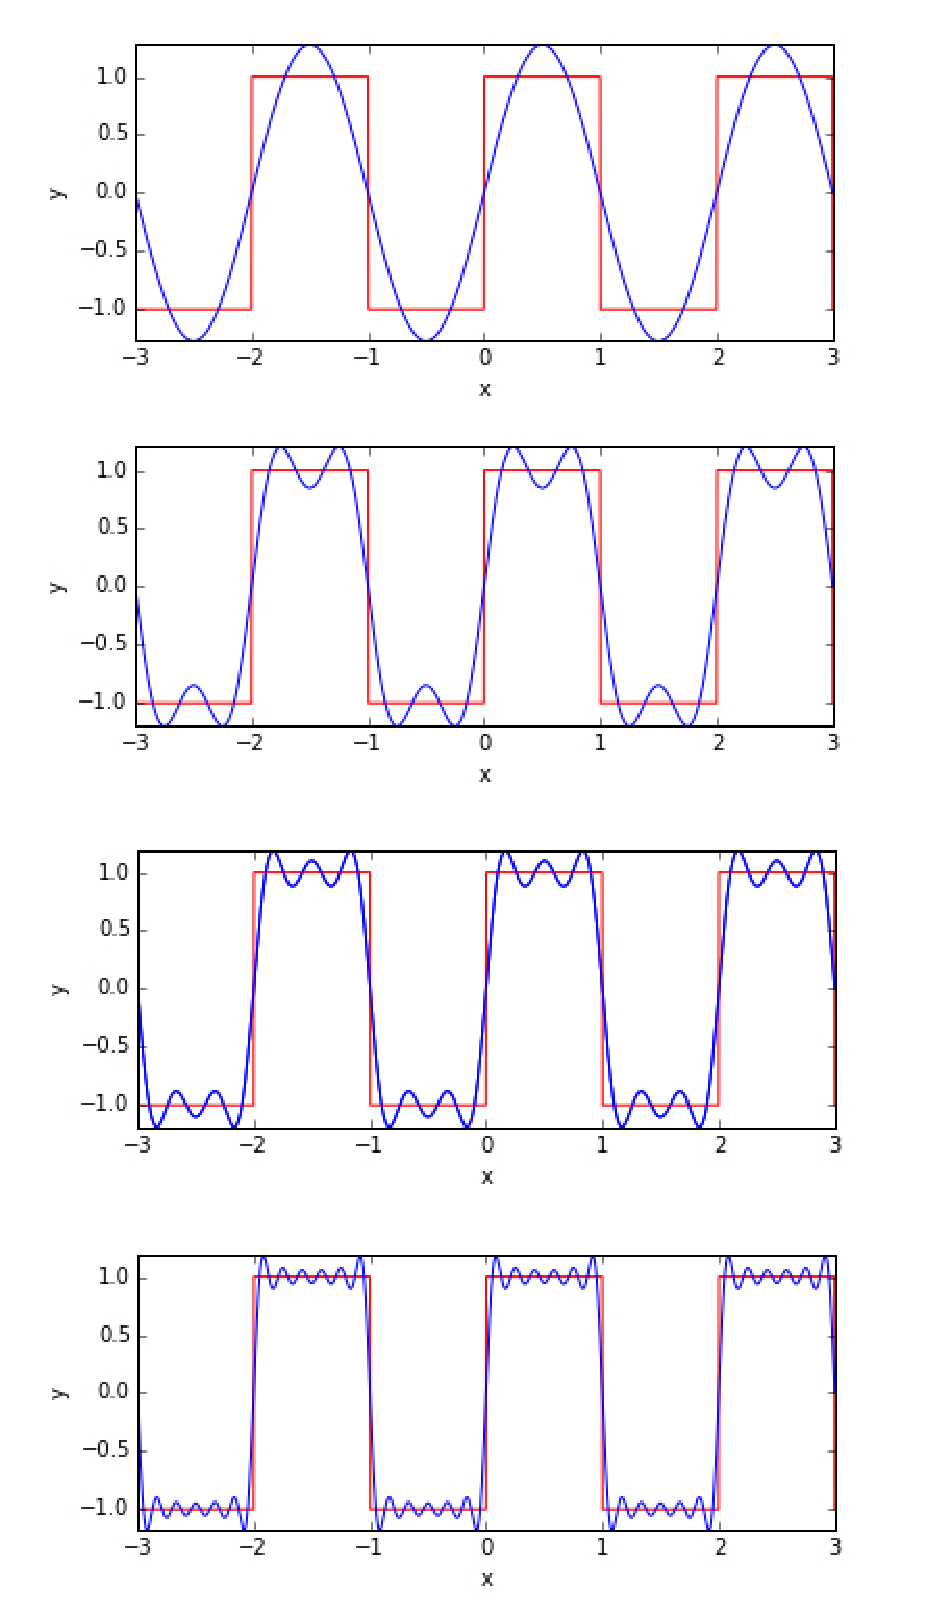
\includegraphics[width=0.40\textwidth]{figs/fsall.pdf}}
\end{center}
\caption{\label{fig:fall} The Fourier Series for a step function including one term, three terms, five terms, and nineteen terms.  The Fourier Theorem states that the series will converge, reproducing the original function, as the number of terms approaches infinity.}
\end{figure}

For a visual example of the Fourier Series, the first terms of the Fourier Series for a step function are shown in Fig.~\ref{fig:fall}.  

\subsection{Determining Fourier Coefficients}
\label{sect:coeff}

Just as in the Euclidean vector space, we can determine the Fourier coefficients of a function $f$ by computing the inner products:
\begin{eqnarray*}
A_n = \braket{c_n| f} \\
B_n = \braket{s_n| f}
\end{eqnarray*}
or, in terms of the inner product integrals and sine and cosine functions:
\begin{eqnarray*}
A_0 &=& \sqrt{\frac{1}{a}} \int_{-\frac{a}{2}}^{\frac{a}{2}} f(x) \, dx \\
A_n &=& \sqrt{\frac{2}{a}} \int_{-\frac{a}{2}}^{\frac{a}{2}} 
\cos\left(\frac{2\pi n}{a} \, x \right) \, f(x) \, dx \\
B_n &=& \sqrt{\frac{2}{a}} \int_{-\frac{a}{2}}^{\frac{a}{2}} 
\sin\left(\frac{2\pi n}{a} \, x \right) \, f(x) \, dx \\
\end{eqnarray*}


The inner product determines the correct coefficients only because the basis functions are complete and orthonormal.  To see how this works, start with the completeness equation but replace $n$ with $m$ for clarity later:
\begin{equation*}
f(x) \; = \; \sum_{m=0}^{\infty}  A_m \, c_m(x)  \; \; + \; \; \sum_{m=1}^{\infty} B_m \, s_m(x)
\end{equation*}
Then calculate:
\begin{eqnarray*}
\braket{c_n| f} \; &=& \; \sum_{m=0}^{\infty}  A_m \, \braket{c_n| c_m}  \; \; + \; \; \sum_{m=1}^{\infty} B_m \, \braket{c_m| s_m} \\[8pt]
 &=& \; \sum_{m=0}^{\infty}  A_m \; \delta_{nm}  \; \; + \; \; \sum_{m=1}^{\infty} B_m \; 0 \\[8pt]
\braket{c_n| f} \; &=& A_n \\
\end{eqnarray*}
Note that the last step follows from the fact that, because of the $\delta_{nm}$ in the product, the only non-zero value in the sum across $m$ is the term for $m=n$.  It is left as an exercise to work this out for $\braket{s_n | f}$.  (It is also helpful to work through these same steps using the integral form of the orthogonality conditions.  It's much more cumbersome notation, but much more explicit about what is going on.  I highly recommend doing this if you are finding the abstract notation confusing at this point.)

\subsection{Application of Fourier Series to Infinite Well}

For the infinite potential well
\begin{equation}
V(x) = 
\begin{cases}    
   0 & 0 \leq x \leq b \\
   +\infty & {\rm otherwise} \\
\end{cases}   
\end{equation}
we have a wave function $\psi(x)$ which meets the boundary conditions $\psi(0) = \psi(b) = 0$.  We define a helper function:
\begin{equation*}
f(x) = 
\begin{cases}    
  \hspace{9.5pt}\psi(x)  & \hspace{9pt} 0 \leq x \leq b \\
  -\psi(-x) & -b \leq x < 0 \\
\end{cases}   
\end{equation*}
It is an odd function by construction:  $f(-x) = -f(x)$.  Since f(b) = f(-b) = 0, we can consider it to be a periodic function with period $2b$. To evaluate it's Fourier series, we'll only need to evaluate it in the region $[-b,b]$ where it is defined\footnote{If you prefer, you can imagine making the helper function truly periodic by just stamping out a copy of $f(x)$ from $[-a,a]$ into $[a,3a]$, and so on.  It will have no effect in what follows.}.  When applying the formulas for the Fourier series, we will need to make the substitute $a \to 2b$ into the original formulas, because the period of $f(x)$ is $2b$.

For $f(x)$ the Fourier coefficients of the cosines all vanish:
\begin{eqnarray*}
A_0 &=& \sqrt{\frac{1}{2b}} \int_{-b}^{b} f(x) \, dx = 0\\
A_n &=& \sqrt{\frac{1}{b}} \int_{-b}^{b} 
\cos\left(\frac{\pi n}{b} \, x \right) \, f(x) \, dx = 0\\
\end{eqnarray*}
and so the Fourier Series for $f(x)$ contains only sines:
\begin{eqnarray*}
f(x) &=& \sqrt{\frac{1}{b}} \sum_{n=1}^{\infty}  B_n \, \sin\left(\frac{\pi n}{b} \, x \right) \\
&=&  \sum_{n=1}^{\infty}  \left( \frac{B_n}{\sqrt{2}}\right) \, \left[ \sqrt{\frac{2}{b}} \, \sin\left(\frac{\pi n}{b} \, x \right) \right]\\
\end{eqnarray*}
Where we have arranged the factors of $\sqrt{2}$ so that the function in square brackets $[\ldots]$ has unit normalization on $[0,b]$.  We determine the Fourier coefficients for the sines from:
\begin{eqnarray*}
B_n &=& \sqrt{\frac{1}{b}} \int_{-b}^{b} 
\sin\left(\frac{\pi n}{b} \, x \right) \, f(x) \, dx = 0\\
\end{eqnarray*}
but since the integrand is now even, the integral does not vanish, and in fact, we need only integrate in $[0,b]$ and multiply by a factor of two:
\begin{eqnarray*}
B_n &=& 2 \times \sqrt{\frac{1}{b}} \int_{0}^{b} 
\sin\left(\frac{\pi n}{b} \, x \right) \, f(x) \, dx = 0\\[14pt]
c_n \equiv \frac{B_n}{\sqrt{2}} &=& \int_{0}^{b} 
\left( \sqrt{\frac{2}{b}} \sin\left(\frac{\pi n}{b} \, x \right) \right) f(x) dx \\
\end{eqnarray*}
And since we are now integrating only from $[0,b]$ then 
$$f(x) = \psi(x)$$ 
and we can rewrite these equations in terms of 
\begin{equation}
\psi_n(x) = 
\begin{cases}
{\displaystyle \sqrt{\frac{2}{b}} \, \sin(k_n x)} & 0 \leq x \leq b\\[8pt]
0 & \rm otherwise \\
\end{cases}
\end{equation}
where
\begin{eqnarray*}
k_n&=&\frac{n\pi}{b}
\end{eqnarray*}
Any wave function in [0,b] can be expressed as a linear combination of these basis functions:
\begin{equation}
\psi(x) = \sum_{n=1}^{\infty} \; c_n \psi_n(x)
\end{equation}
and
\begin{eqnarray*}
c_n &=& \braket{\psi_n| \psi} = \int_{0}^{b} \; \psi_n(x) \, \psi(x) \, dx \\
\end{eqnarray*}

\section{Insights from the Infinite Square Well}

Let's recap what we have learned so far.  By assuming that we could find solutions of the form
\begin{eqnarray*}
\Psi(x,t) = \psi(x) \, \phi(t)
\end{eqnarray*}
we have indeed found an infinite number of solutions to the TISE for the Infinite Square Well potential:
\begin{equation*}
\hat{H} \, \psi_n(x) = E_n \, \psi_n(x)
\end{equation*}
for $n=1,2,3,\dots$. Each of these solutions has an associated time dependent ``wiggle factor'':
\begin{equation*}
\phi_n(t) = \exp(-\frac{i E_n t}{\hbar})
\end{equation*}
so that the total wave equation is:
\begin{equation*}
\Psi_n(x,t) = \exp(-\frac{i E_n t}{\hbar}) \, \psi_n(x)
\end{equation*}
We saw that these are {\bf stationary states} (the expectation values are constant in time) and they are {\bf states of definite energy} (every measurement of their energy will yield the results $E_n$).

The wave functions $\Psi_n(x,t)$ are solutions to the (time dependent) SE.  It's instructive to see exactly how that works:
\begin{eqnarray*}
\hat{H} \, \Psi_n(x,t) &=& -\ihbar \frac{\partial\Psi}{\partial t}\\[8pt]
\exp(-\frac{i E_n t}{\hbar}) \; \hat{H} \; \psi_n(x) &=& -\ihbar \psi_n(x) \, \frac{d}{dt}
\exp(-\frac{i E_n t}{\hbar})\\[8pt]
\exp(-\frac{i E_n t}{\hbar}) \; E_n \; \psi_n(x) &=& -\ihbar \psi_n(x) \, \frac{-iE_n}{\hbar}
\exp(-\frac{i E_n t}{\hbar})\\[8pt]
E_n \Psi(x,t) &=& E_n \Psi(x,t)\\[8pt]
\end{eqnarray*}
The recognition of stationary states as the Fourier series gives us a crucial additional insight.  The $\psi_n(x)$ are also a complete orthonormal basis (the Fourier series) for any function that meets the boundary conditions for this problem.  That means that we have in fact already found the {\em general solution} to this problem.

Let's see how this works.  Suppose the initial state of a particle is $\Psi(x,0) \equiv \psi_i(x)$.  This can be absolutely any function so long as it vanishes outside of $[0,a]$ and it is properly normalized.  Our job is to find $\Psi(x,t)$ that satisfies the SE for all future times.  We calculate the Fourier coefficients of $\psi_i(x)$ as:
\begin{eqnarray*}
c_n &=& \braket{\psi_n| \psi_i} = \int_{0}^{a} \; \psi_n(x) \, \psi_i(x) \, dx \\
\end{eqnarray*}
and by Fourier's theorem, we know that:
\begin{eqnarray*}
\Psi(x,0) &=& \sum_{n=0}^{\infty} c_n \, \psi_n(x)
\end{eqnarray*}
But what about $\Psi(x,t)$?  It really couldn't be any simpler:
\begin{equation*}
\Psi(x,t) \; = \; \sum_{n=0}^{\infty} c_n \, \Psi_n(x,t) \; = \; \sum_{n=0}^{\infty} c_n \, \exp(-\frac{i E_n t}{\hbar}) \, \psi_n(x)
\end{equation*}
It is left as an exercise to show explicitly that $\Psi(x,t)$ as defined here does satisfy the time-dependent SE and is equal to $\psi_i(x)$ at $t=0$. 

There is still some insight to be gleamed from this simple example.  We specified that $\Psi(x,0)$ is normalized, and we showed that the SE preserves normalization, so we know that $\Psi(x,t)$ is normalized as well:
\begin{equation*}
\int_{-\infty}^{+\infty} |\Psi(x,t)|^2 \; dx = 1
\end{equation*}
And plugging in the Fourier series for $\Psi(x,t)$:
\begin{eqnarray*}
1 &=& \int_{-\infty}^{+\infty} \Psi^*(x,t)\Psi(x,t) \; dx \\
  &=& \int_{-\infty}^{+\infty} \left( \sum_{n=1}^{\infty} c_n^* \Psi_n^*(x,t) \right) \left( \sum_{m=1}^{\infty} c_m \Psi_m(x,t) \right) \; dx \\
  &=& \sum_{n=1}^{\infty} \; \sum_{m=1}^{\infty} \; c_n^* c_m  \, \exp\left(\frac{i(E_n-E_m)t}{\hbar}\right) \int_{-\infty}^{+\infty} \psi_n^*(x) \psi_m(x) \; dx \\
  &=& \sum_{n=1}^{\infty} \; \sum_{m=1}^{\infty} \; c_n^* c_m  \, \exp\left(\frac{i(E_n-E_m)t}{\hbar}\right) \delta_{nm} \\
\end{eqnarray*}
so that  
\begin{equation}  
\sum_{n=1}^{\infty} |c_n|^2 = 1
\end{equation}
We can also calculate:
\begin{eqnarray*}
\braket{H} &=& \int_{-\infty}^{+\infty} \Psi^*(x,t)\hat{H}\Psi(x,t) \; dx \\
  &=& \int_{-\infty}^{+\infty} \left( \sum_{n=1}^{\infty} c_n^* \Psi_n^*(x,t) \right) \hat{H}\left( \sum_{m=1}^{\infty} c_m \Psi_m(x,t) \right) \; dx \\
  &=& \sum_{n=1}^{\infty} \; \sum_{m=1}^{\infty} \; c_n^* c_m \, \exp\left(\frac{i(E_n-E_m)t}{\hbar}\right) \int_{-\infty}^{+\infty} \psi_n^*(x) \hat{H} \psi_m(x) \; dx \\
  &=& \sum_{n=1}^{\infty} \; \sum_{m=1}^{\infty} \; c_n^* c_m \, \exp\left(\frac{i(E_n-E_m)t}{\hbar}\right) \int_{-\infty}^{+\infty} \psi_n^*(x) E_m \psi_m(x) \; dx \\
  &=& \sum_{n=1}^{\infty} \; \sum_{m=1}^{\infty} \; c_n^* c_m \, \exp\left(\frac{i(E_n-E_m)t}{\hbar}\right) E_m \int_{-\infty}^{+\infty} \psi_n^*(x) \psi_m(x) \; dx \\
  &=& \sum_{n=1}^{\infty} \; \sum_{m=1}^{\infty} \; c_n^* c_m  \, \exp\left(\frac{i(E_n-E_m)t}{\hbar}\right) E_m \delta_{nm} \\
\end{eqnarray*}

so that  
\begin{equation}  
\braket{H} = \sum_{n=1}^{\infty} |c_n|^2 E_n
\end{equation}
Recall from our review of statistics that:
\begin{equation}  
\braket{H} = \sum_{n=1}^{\infty} P(n) E_n
\end{equation}
where $P(n)$ is the probability of observing the particle in state $n$.  This allows us to identify $|c_n|^2$ as the probability of observing the particle with energy $E_n$.

At this point, it would be reasonable to assume that these results apply only to the infinite square well potential.  In fact, there is a generalization to the Fourier series called the Spectral Theorem which shows that these results apply more more widely.  The stationary solutions to the TISE will always be a complete orthonormal basis for the general solution, exactly as here. 


\section{Commutators}

Let's review the situation.  The state of a quantum system is contained entirely in a wave function $\Psi(x,t)$ which is a function of the position $x$ but not momentum $p$.  To calculate quantities involving momentum, instead of a variable, we must use the momentum operator:
$$\hat{p} = -i \hbar \frac{\partial}{\partial x}$$
But note that while:
$$ x \, \hat{p} \; \Psi(x, t) = -\ihbar \, x \frac{\partial \Psi}{\partial x}$$
because of the chain rule, we have:
$$ \hat{p} \, x \; \Psi(x, t) = -\ihbar \Psi(x,t) - \ihbar \, x \frac{\partial \Psi}{\partial x}$$
and:
$$ \left( x \, \hat{p} - \hat{p} \, x \right) \, \Psi(x, t) = \ihbar \, \Psi(x,t) $$
This might seems like it is all a silly mistake... like maybe we should just be more careful with our parenthesis in our notation and apply operators only to the part we want without getting anything extra.  But no, this non-commutative behavior and its physical consequences are far reaching and impossible to avoid.

When using operators we encounter terms like $x\hat{p} - \hat{p}x$ so often that we have a special notation for them.  The commutator of $A$ and $B$ is written and defined as:
\begin{equation}
\label{eqn:commutator}
\left[\hat{A}, \hat{B}\right] = \hat{A} \hat{B} - \hat{B} \hat{A} 
\end{equation}
Using this notation, and noting $\hat{x}=x$, we can rewrite our result about as:
$$ \left[ \hat{x} , \hat{p} \right] \, \Psi(x, t) = \ihbar \, \Psi(x,t) $$
or more simply:
\begin{equation}
\label{eqn:pxcom}
\left[\hat{x}, \hat{p}\right] = i \hbar 
\end{equation}
This small little equation is called the {\bf canonical commutation relation} and as we will see, it is a central feature of quantum mechanics.

\section{The Harmonic Oscillator}

The classical harmonic oscillator is a mass $m$ connected to a spring which follows Hooke's law:
\begin{equation*}
F = -k \, x = m \frac{d^2x}{dt^2} 
\end{equation*}
with oscillatory solutions
\begin{equation*}
x(t) = A \cos(\omega t) + B \sin(\omega t)
\end{equation*}
where:
\begin{equation*}
\omega = \sqrt{\frac{k}{m}}
\end{equation*}
The potential energy is
\begin{equation*}
V(x) = \frac{1}{2}k x^2 = \frac{1}{2} m \omega^2 x^2
\end{equation*}
The classical harmonic oscillator is {\em widely} applicable, at least as an approximation, because any potential is approximately a parabola near a local minimum in the potential:
\begin{eqnarray*}
V(x) &=& V(x_0) + V'(x_0) \, (x-x_0) + \frac{1}{2}\,V''(x_0) \, (x-x_0)^2 + \ldots \\[5pt]
V(x) &=& V_0 + \frac{1}{2}\,V''(x_0) \, (x-x_0)^2 + \ldots \\[5pt]
V(x) &\approx& -\frac{1}{2}\,V''(x_0)\\
\end{eqnarray*}
where we have used the fact that $V'(x_0)=0$ at the minimum and the constant offset $V_0$ can be taken as zero.

In this section, we will turn our attention to the widely applicable quantum harmonic oscillator, and find the solutions to the TISE for:
\begin{equation*}
\hat{H} = -\frac{\hbar^2}{2m}\,\frac{\partial^2}{\partial x^2} + \frac{1}{2} m \omega^2 x^2
\end{equation*}
We are first going to solve this the hard way, through the power series solution, and then solve it using an elegant algebraic method.

\subsection{Power Series Solutions}

We are solving this equation:
\begin{equation*}
-\frac{\hbar^2}{2m}\,\frac{d^2 \psi}{d x^2} + \frac{1}{2} m \omega^2 x^2 \psi(x) = E \psi(x)
\end{equation*}
but if we leave it in that form we will spend all our time dealing with constants and not make any progress.  Instead our idea is two multiply through by:
$$\frac{2}{\hbar \omega}$$
as this will make the coefficient of the RHS dimensionless, and get rid of the factors of $1/2$ on the LHS.  This gives us:
\begin{equation*}
-\frac{\hbar}{m\omega}\,\frac{d^2 \psi}{d x^2} + \frac{m \omega}{\hbar} x^2 \psi(x) = \frac{2E}{\hbar\omega} \psi(x)
\end{equation*}
and we can see the progress we've made if we put:
$$x_0 \equiv \sqrt{\frac{\hbar}{m \omega}}$$ 
and 
$$\epsilon \equiv \frac{2E}{\hbar\omega} $$
Our equation becomes:
\begin{equation*}
-x_0^2 \; \frac{d^2 \psi}{d x^2} \, + \, \frac{x^2}{x_0^2} \, \psi(x) \; = \; \epsilon \, \psi(x)
\end{equation*}
which is already looking less tedious.  But note that we can define a dimensionless variable $u$ to replace $x$ as:
$$u \equiv \frac{x}{x_0}$$
and noting that:
$$\frac{d}{dx} = \frac{du}{dx}\frac{d}{du} = a \frac{d}{du}$$
we have at last:
\begin{equation*}
-\frac{d^2 \psi}{d u^2} \, + \, u^2 \, \psi(u) \; = \; \epsilon \, \psi(x)
\end{equation*}
or:
\begin{equation*}
\frac{d^2 \psi}{d u^2} \; =  \; (u^2 - \epsilon) \, \psi(u) 
\end{equation*}
the same equation with the tedious constants hidden in our variable definitions.

Next we consider the behavior of $\psi$ at large $u$ (which is also large $x$).  In this case, the differential equation becomes:
\begin{equation*}
\frac{d^2 \psi}{d u^2}  \approx u^2 \psi(u) 
\end{equation*}
Noticing that the derivatives cause the power of $u$ to increase leads us to try something like:
\begin{equation*}
\psi(u) = \exp\left(\frac{\alpha u^2}{2}\right)
\end{equation*}
for some $\alpha$, because each derivative will bring down a factor of $u$.  But as we'll see, even something like:
\begin{equation*}
\psi(u) = u^k \; \exp\left(\frac{\alpha u^2}{2}\right)
\end{equation*}
will do the trick.  Trying it out:
$$\frac{d \psi}{d u}  = \left(\alpha u^{k+1} + k\,u^{k-1}\right) \, \exp\left(\frac{\alpha u^2}{2}\right) $$
and
$$\frac{d^2 \psi}{d u^2}  = \alpha^2 u^{k+2} \exp\left(\frac{\alpha u^2}{2}\right) \, \left(1 + \mathcal{O}(1/u^2)\right)$$
where the symbol $\mathcal{O}(1/u^2)$ means terms of order $1/u^2$ and smaller.  Because $u$ is large, we can neglect these higher order terms relative to the leading 1, and get:
$$\frac{d^2 \psi}{d u^2}  = \alpha^2 u^2 \psi$$
which satisfies the differential equation if $\alpha^2 = 1$, i.e.:
$$\psi(u) = A u^k \exp(-u^2/2) + B u^k \exp(+u^2/2)$$
but we cannot hope to normalize the wave function unless the $B$ term is zero.  So we conclude that the limiting behavior of the wave function we want is:
$$\psi(u) = A u^k \exp(-u^2/2)$$
This leads us to try a solution of the form:
$$\psi(u) = h(u) \exp(-u^2/2)$$
where $h(u)$ is any function of $u$.  Note that we are no longer making any approximation.  We can express any wave function this way.  We are just hopeful the differential equation for $h(u)$ will be easier to solve than the differential equation for $\psi(u)$, because the asymptotic behavior has been factored out.  Trying it out:
$$\frac{d\psi}{du} = \left( \frac{dh}{du} - u\, h(u)\right) \, e^{-u^2/2}$$
and
$$\frac{d^2\psi}{du^2} = \left( \frac{d^2h}{du^2} - 2 u \frac{dh}{du} + (u^2-1)h(u) \right) \, e^{-u^2/2}$$
the TISE becomes:
\begin{eqnarray*}
\left( \frac{d^2h}{du^2} - 2 u \frac{dh}{du} + (u^2-1)h(u) \right) \, e^{-u^2/2} &=& (u^2-\epsilon)\\[7pt] 
\left( \frac{d^2h}{du^2} - 2 u \frac{dh}{du} + (\epsilon-1)h(u) \right) \, e^{-u^2/2} &=& 0\\
\end{eqnarray*}
but $e^{-u^2/2}$ is nowhere zero, so we are left with the TISE for $h(u)$ as:
\begin{equation}
\label{eqn:htise}
\frac{d^2h}{du^2} - 2 u \frac{dh}{du} + (\epsilon-1)h(u) = 0
\end{equation}
We will solve it with everyones least favorite method: power series.  We assume:
$$h(u) = \sum_{m=0}^{\infty} a_m u^m$$
then calculate:
$$\frac{dh}{du} = \sum_{m=0}^{\infty} m a_m u^{m-1}$$
and
$$\frac{d^2h}{du^2} = \sum_{m=0}^{\infty} m (m-1) a_m u^{m-2}$$
Then we start collecting terms from the LHS of the Equation~\ref{eqn:htise}:
$$(\epsilon-1)\;h(u) = \sum_{m=0}^{\infty} (\epsilon-1)\;a_m u^m$$
and:
$$-2 u \, \frac{dh}{du} = \sum_{m=0}^{\infty} -2 \, m \, a_m \, u^{m}$$
which to our good fortune have the same power of $u$ for each value of $m$.  But that is not the case for the second derivative, which we will reproduce here as:
$$\frac{d^2h}{du^2} = \sum_{n=2}^{\infty} n (n-1) a_n u^{n-2}$$
with the index in the sum changed to $n$ (for simplicity below) and where the first two terms have been omitted from the sum as they are both zero.  To line up nicely with the first two series, we need to have the term $m$ be a power $u^m$ so substituting $m = n - 2$ we get:
$$\frac{d^2h}{du^2} = \sum_{m=0}^{\infty} (m+2) (m+1) a_{m+2} u^{m}$$
and the TISE for $h(u)$ becomes:
$$\sum_{m=0}^{\infty} \left[(\epsilon-1)\;a_m -2 \, m \, a_m + (m+2) (m+1) a_{m+2} \right] u^{m} = 0$$
to be zero everywhere, the coefficients of every power of $u$ must vanish, leading to:
$$(\epsilon-1)\;a_m -2 \, m \, a_m + (m+2) (m+1) a_{m+2} = 0$$
which can be written as the recursion relationship:
$$a_{m+2} = \frac{2m+1-\epsilon}{(m+2)(m+1)} \; a_m$$
which appears on a first glance to solve the problem.  This recursion relation will give all the even $a_m$ starting from $a_0$ and all the odd $a_m$ starting from $a_1$. Noting that:
$$h(0) = a_0$$
and 
$$h'(0) = a_1$$
it seems that given two initial conditions, we obtain the corresponding solution $h(u)$ as a series.  
We can break this solution into two solutions, an even solution and an odd solution:
$$h(u) = h_{\rm even}(u) + h_{\rm odd}$$
with:
$$h_{\rm even}(u) = a_0 + a_2 \, u^2 + a_4 \, u^4 + \ldots$$
and 
$$h_{\rm odd}(u) = a_1 \, u + a_3 \, u^3 + a_5 \, u^5 + \ldots$$

But on a closer look, it seems we are in deep trouble for two reason.  First, we expected (as in the infinite square well) to find that we had solutions only for certain values of the energy ($epsilon$ here) but these recursion relations give a solution for any value of $\epsilon$.  Secondly, for large $m$ the recursion relationship becomes:
$$a_{m+2} \approx \frac{2}{j}\;a_{m}$$
which looks like {\bf bad news}.  Let's start with $h_{\rm even}(u)$.  Picking some large even number $2n$ and defining (you see why shortly):
$$C \equiv a_{2n} n!$$
we have:
$$a_{2(n+1)} \approx \frac{1}{n}\;a_{2n} \approx \frac{1}{n+1}\;a_{2n} = \frac{C}{(n+1)!}$$
and it keeps going:
$$a_{2(n+2)} \approx \frac{C}{(n+2)!}$$
So the asymptotic behavior of $h_{\rm even}$ is:
$$h_{\rm even}(u) \approx \sum_{n=0}^{\infty} \frac{C}{n!}u^{2n} = C\exp(u^2)$$
and so:
$$\psi(u) \approx h_{\rm even}(u) \exp(-u^2/2) \approx C \exp(u^2/2)$$
which we cannot possibly normalize.  In fact, this is {\bf exactly} the unusable solution to the TISE at large $u$ that we threw away, coming back to us.
You might hope that $h_{\rm odd}(u)$ can save the day, but we can pick a large odd number $2n+1$ and proceed in exact same manner to find that $h_{\rm odd}(u)$

There is only one way out of this predicament.  The series must terminate at some coefficient $a_n$.
Looking back at Equation~\ref{eqn:hermite-recursion} we see that if:
$$2n+1-\epsilon = 0$$
then $a_{n+2} = 0$.  Recalling our definition for $\epsilon$ we see that:
\begin{equation}
E = \hbar \omega \left( n + \frac{1}{2} \right)
\end{equation}
The highest power term in the series defining $h(u)$ will be $u^n$, with the asymptotic before of $\psi(u)$ now:
$$\psi(u) \; \approx \; h(u) \, \exp(-u^2/2) \; \approx \; C \, u^n \, \exp(-u^2/2)$$
this is precisely the nice behavior we choose at the very start.

We can work out explicit solutions.  It's convenient to rewrite the recursion formula in terms of the quantum number $n$ instead of $\epsilon = 2n+1$:
\begin{equation}
a_{m+2} = \frac{-2(n-m)}{(m+2)(m+1)} \; a_m
\end{equation}
For $n=0$, the last term is $a_0$, so we have simply
$h_0(u) = a_0$ and so
$$\psi_0(u) = a_0 e^{-u^2/2}$$
For $n=1$, the last term is $a_1$, and so $h_1=a_1 u$ and
$$\psi_1(u) = a_1 u e^{-u^2/2} $$
For $n=2$, the last term is $a_2$, with $a_2 = -2a_0$ and so
and so $h_2=a_0 \, (1-2u^2)$ and
$$\psi_2(u) =  a_0 \, (1-2u^2) \, e^{-u^2/2} $$

The polynomials are know as the Hermite polynomials $H_n(u)$.  They can be most ``easily'' obtained from the Taylor expansion of the generating function:
$$\exp(-z^2+2zu) = \sum_{n=0}^{\infty} \frac{z_n}{n!}H_n(u)$$
with this convention, the normalized stationary states for the harmonic oscillator are:
$$\psi_n(x) = \left( \frac{m \omega}{\pi \hbar} \right)^{1/4} \frac{1}{\sqrt{2^n n!}}H_n(u) e^{-u^2/2}$$
where
$$u \equiv \sqrt{\frac{m \omega}{\hbar}} x$$.

 
\subsection{Algebraic Method}

We write the Hamiltonian for the harmonic oscillator in terms of the position and momentum operators:
\begin{equation*}
\hat{H} = \frac{1}{2m}\,\left[ \hat{p}^2 + \left( m \omega \hat{x} \right)^2 \right]
\end{equation*}
In this problem, the only parameter is $\omega$, the frequency of the classical harmonic oscillator, and so $\hbar \omega$ has units of energy. It's reasonable to consider the dimensionless quantity:
\begin{equation*}
\frac{\hat{H}}{\hbar\omega} \; = \; \frac{\hat{p}^2 + (m \omega \hat{x})^2 }{2 \hbar m \omega }
\; = \; \frac{1}{2} \, \left( \left(\frac{\hat{p}}{p_0}\right)^2 + \frac{m \omega \hat{x}^2 }{\hbar} \right)
\end{equation*}
As before, we define:
$$x_0 \equiv \sqrt{\frac{\hbar}{m \omega}}$$
and also:
$$p_0 \equiv \frac{\hbar}{x_0} = \sqrt{\hbar m \omega}$$
so:
\begin{equation*}
\frac{\hat{H}}{\hbar\omega} \; = \; \frac{1}{2} \, \left[ \left(\frac{\hat{p}}{p_0}\right)^2 + \left( \frac{\hat{x}}{x_0}\right)^2 \right]
\end{equation*}
The algebraic solution we will use here is based on the observation that we can factor the dimensionless product in square brackets.  If these were ordinary real numbers we would have:
$$\alpha^2 + \beta^2 = (\alpha + i\beta) \, (\alpha - i\beta) $$
so we'll define:
\begin{eqnarray*}
\hat{a}_- &\equiv& \frac{1}{\sqrt{2}}\left(i \frac{\hat{p}}{p_0} + \frac{\hat{x}}{x_0}\right) \\
\hat{a}_+ &\equiv& \frac{1}{\sqrt{2}}\left(-i \frac{\hat{p}}{p_0} + \frac{\hat{x}}{x_0} \right) \\
\end{eqnarray*}
there are other possible choices for the sign and which term is made imaginary, and these would work as well in what follows, but this choice will give us the most conventional notation for our results.  We calculate:

\begin{eqnarray*}
\hat{a}_{+}\, \hat{a}_{-} \; &=& \; \frac{1}{2} \left[
\left( \frac{\hat{p}}{p_0}\right)^2 \; + \; \left( \frac{\hat{x}}{x_0}\right)^2
+ i \, \frac{\hat{x}\hat{p} - \hat{p}\hat{x}}{x_0 \, p_0}
\right] \\[8pt]
&=& \; \frac{\hat{H}}{\hbar \omega} \; + i \, \frac{[\hat{x},\hat{p}]}{\hbar}
\end{eqnarray*}
where we have noted that $x_0 p_0 = \hbar$.  Using the canonical commutation relation $[\hat{x}, \hat{p}] = i\hbar$:
\begin{equation*}
\hat{a}_{+}\,\hat{a}_{-} \; = \; \frac{\hat{H}}{\hbar\omega} \; - \frac{1}{2}
\end{equation*}
and a similar calculation gives:
\begin{equation*}
\hat{a}_{-}\,\hat{a}_{+} \; = \; \frac{\hat{H}}{\hbar\omega} \; + \frac{1}{2}
\end{equation*}
so that:
\begin{equation}
\label{eqn:ladder-com}
[\hat{a}_-, \hat{a}_+] \; = \; \hat{a}_- \, \hat{a}_+ - \hat{a}_+, \hat{a}_- \; = \;  1
\end{equation}
and
\begin{equation}
\label{eqn:ladder-ham}
\hat{H} =  \hbar\omega \left( \hat{a}_+ \hat{a}_- + \frac{1}{2} \right)
\end{equation}
These two equations contain everything that we need.  Let's start by calculating:
\begin{eqnarray*}
[\hat{H}\,,\,\hat{a}_+] &=& \hbar \omega \; [\hat{a}_+ \hat{a}_-, \hat{a}_+]  \\
&=& \hbar \omega \; \left( \hat{a}_+ \hat{a}_- \hat{a}_+ - \hat{a}_+ \hat{a}_+ \hat{a}_- \right) \\
&=& \hbar \omega \; \hat{a}_+ (\hat{a}_- \hat{a}_+ - \hat{a}_+ \hat{a}_-)\\
&=& \hbar \omega \; \hat{a}_+ [\hat{a}_-, \hat{a}_+]\\
&=& \hbar \omega \; \hat{a}_+ 
\end{eqnarray*}
Similarly
\begin{equation*}
[\hat{H},\hat{a}_-] = -\hbar \omega 
\end{equation*}
So now suppose we have a solution to the TISE, so that:
$$\hat{H} \Psi = E \Psi$$
then we also have:
\begin{eqnarray*}
\hat{H} \left( \hat{a}_+ \Psi \right) &=& \left( \hat{H} \hat{a}_+ \right) \; \Psi\\
     &=& \left( \hat{H} \hat{a}_+ \; - \; \hat{a}_+ \hat{H} \; + \; \hat{a}_+ \hat{H} \right) \; \Psi\\
     &=& \left( [\hat{H}, \hat{a}_+] \; + \; \hat{a}_+ \hat{H} \right) \; \Psi\\
     &=& \left( \hbar\omega \, \hat{a}_+ \; + \; \hat{a}_+ \hat{H} \right) \; \Psi\\
     &=& \left( \hbar\omega \, \hat{a}_+ \; + \; \hat{a}_+ \, E \right) \; \Psi\\
     &=& \left( E \; + \; \hbar\omega \right) \; (\hat{a}_+ \, \Psi)\\
\end{eqnarray*}
which shows that $\hat{a}_+ \Psi$ is a new solution to the TISE with energy $E+\hbar\omega$.  A similar calculation shows that:
$$\hat{H} \left(\hat{a}_-\Psi\right) = \left( E - \hbar \omega \right) \left(\hat{a}_-\Psi\right)$$
that is $\hat{a}_- \Psi$ is a new solution to the TISE with energy $E+\hbar\omega$.

So evidently, given even one solution to the TISE, we can find an infinite number of new states at higher energy by successive applications of $\hat{a}_+$.  But what of $\hat{a}_-$?  We know that the energy of a normalizable wave function must be greater than zero.  So there must be a ground state, let's call it $\Psi_0$ such that:
\begin{equation}
\hat{a}_- \Psi_0 = 0
\end{equation}
What is the energy of the ground state?  We can ``ask'' the Hamiltonian:
\begin{eqnarray*}
\hat{H} \psi_0 &=& \hbar\omega \left( a_+ a_- + \frac{1}{2} \right) \psi_0 \\
&=& \frac{\hbar\omega}{2}\psi_0 + \hbar\omega a_+ \left( a_- \psi_0 \right)\\
&=& \frac{\hbar\omega}{2}\psi_0\\
\end{eqnarray*}
So the ground state has energy $E_0 = \hbar\omega/2$ and we have:
\begin{equation}
E_n = \hbar \omega \left(n + \frac{1}{2} \right) \hspace{3cm} n = 0,1,2,\ldots
\end{equation}
Take a look back at what a different way of doing business this has been.  We have determined the entire energy spectrum from Equations \ref{eqn:ladder-com} and \ref{eqn:ladder-ham} using nothing but  algebra.

Let's see how far we can take this.
\begin{eqnarray*}
\hat{H} \psi_n &=& E_n \psi_n \\
\hbar\omega \left( a_+ a_- + \frac{1}{2} \right) \psi_n &=& \hbar \omega \left(n + \frac{1}{2} \right) \psi_n \\
\hat{a}_+ \hat{a}_- \psi_n &=& n \psi_n \\
\end{eqnarray*}
Also:
\begin{eqnarray*}
\hat{a}_- \hat{a}_+ \psi_n &=& \left(\hat{a}_+\hat{a}_- + [\hat{a}_-,\hat{a}_+]\right) \psi_n \\
&=& (n+1) \psi_n
\end{eqnarray*}
From their definition, we have:
\begin{equation*}
\hat{x} = \frac{x_0}{\sqrt{2}} \left( a_+ + a_-\right)
\end{equation*}
and 
\begin{equation*}
\hat{p} = \frac{i\,p_0}{\sqrt{2}} \left( a_+ - a_-\right)
\end{equation*}
So we can calculate:
\begin{equation*}
x^2 = \frac{x_0^2}{2} \left( a_+^2 + a_+a_- + a_-a_+ + a_-^2 \right)
\end{equation*}
and so:
\begin{equation*}
V(x) = \frac{1}{2}m \omega^2 x^2= \frac{\hbar \omega}{4} \left( a_+^2 + a_+a_- + a_-a_+ + a_-^2 \right)
\end{equation*}
with
\begin{eqnarray*}
\braket{V} &=& \frac{\hbar \omega}{4} \int_{-\infty}^{+\infty} \psi_n^* \left( a_+^2 + a_+a_- + a_-a_+ + a_-^2 \right) \psi_n \, dx
\end{eqnarray*}
This integral vanishes:
$$\int_{-\infty}^{+\infty} \psi_n^* a_+^2 \psi_n dx = k \int_{-\infty}^{+\infty} \psi_n^* \psi_{n-2} dx
 = 0 $$
as does the integral involving $a_-^2$ leaving only:
\begin{equation*}
\braket{V} = \frac{\hbar \omega}{4} (n + n + 1) = \frac{\hbar \omega}{2} \left(n + \frac{1}{2}\right) 
= \frac{E_n}{2}
\end{equation*}
In principle we can calculate any classical dynamical variable in terms of the a's.


\section{Fourier Series for Complex Functions}

The Fourier series for a periodic function with period $a$ can be expressed in terms of the complex exponential by noting that:
\begin{eqnarray*}
\sin\theta \; = \; \frac{e^{i \theta} - e^{-i \theta}}{2i} \\[5pt]
\cos\theta \; = \; \frac{e^{i \theta} + e^{-i \theta}}{2} \\
\end{eqnarray*}
so:
\begin{eqnarray*}
s_n(x) \; &=& \; \sqrt{\frac{2}{a}} \; \sin\left(\frac{2\pi n x}{a}\right) \; = \; \frac{e_n(x) - e_n^*(x)}{i \sqrt{2}}\\[8pt]
c_n(x) \; &=& \; \sqrt{\frac{2}{a}} \; \cos\left(\frac{2\pi n x}{a}\right) \; = \; \frac{e_n(x) + e_n^*(x)}{\sqrt{2}}\\
\end{eqnarray*}
where:
\begin{equation}
e_n(x) \equiv \frac{1}{\sqrt{a}}\exp\left( i \, \frac{2 \pi n x}{a}\right)
\end{equation}
and note that:
$$c_0(x) = e_0(x)$$
So now the Fourier series for f(x) can be written:
\begin{eqnarray*}
f(x) &=& A_0 c_0(x) + \sum_{n=1}^{\infty}  \left\{ A_n \, c_n( x ) + B_n \, s_n( x ) \right\} \\
&=& A_0 e_0(x) + \sum_{n=1}^{\infty}  \left\{ A_n \,  \frac{e_n(x) + e_n^*(x)}{\sqrt{2}}
+ B_n \,  \frac{e_n(x) - e_n^*(x)}{i\sqrt{2}} \right\} \\
&=& A_0 e_0(x) + \sum_{n=1}^{\infty}  \left\{ \frac{A_n - i B_n}{\sqrt{2}}\, e_n(x) + 
\frac{A_n + i B_n}{\sqrt{2}}\, e_n^*(x)\right\} \\
\end{eqnarray*}
If we define the complex Fourier Coefficient
$$c_n \equiv \frac{A_n-iB_n}{\sqrt{2}}  \hspace{4cm} n=1,2,3,\ldots$$
and put $c_0 \equiv A_0$ then we have:
\begin{eqnarray*}
f(x) &=& c_0 e_0(x) + \sum_{n=1}^{\infty}  \left\{ c_n \, e_n(x) + c_n^* \, e_n^*(x) \right\} \\
\end{eqnarray*}
Furthermore, if we note that:
$$e_{-n}(x) = e_{n}^*(x)$$
and define:
\begin{equation}
\label{eqn:cofreal}
c_{-n} \equiv c_n^*
\end{equation}
we can write this all quite compactly:
\begin{equation*}
f(x) = \sum_{n=-\infty}^{\infty}  c_n \, e_n(x)  \\
\end{equation*}
Now we need only work out how to calculate the complex Fourier coefficients $c_n$. For $n>0$ we had
\begin{eqnarray*}
c_n &\equiv& \frac{A_n - i B_n}{\sqrt{2}}. \\
&=& \frac{1}{\sqrt{2}} \left\{ 
\sqrt{\frac{2}{a}} \int_{-\frac{a}{2}}^{\frac{a}{2}}  f(x) \cos\left( \frac{2\pi n x}{a}\right) \, dx
-i \frac{2}{a} \int_{-\frac{a}{2}}^{\frac{a}{2}}  f(x) \sin\left(\frac{2\pi n x}{a}\right) \, dx
\right\} \\
&=& \frac{1}{\sqrt{a}} \int_{-\frac{a}{2}}^{\frac{a}{2}}  f(x) \left\{\cos\left( \frac{2\pi n x}{a}\right) - i \sin\left( \frac{2\pi n x}{a}\right)\right\} \, dx \\
 &=& \int_{-\frac{a}{2}}^{\frac{a}{2}}  f(x) \; \frac{1}{\sqrt{a}}\exp\left(-i \frac{2\pi n x}{a}\right) \, dx \\
\end{eqnarray*}
or finally:
\begin{equation*}
c_n = \int_{-\frac{a}{2}}^{\frac{a}{2}}  f(x) \; e_n^*(x) \, dx 
\end{equation*}
What's going on?  It seems that to calculate the Fourier coefficient of the $e_n(x)$ we have to use it's complex conjugate $e_n^*(x)$ in the integral with $f(x)$. But we also expect to obtain these coefficients from the inner product of $f(x)$ and $e_n(x)$.  The conclusion is that the definition of the inner product for a vector space of a complex scalar field must include complex conjugation.  For $f(x), g(x) \in \mathbb{C}$ we have:
\begin{equation}
\label{eqn:compips}
\braket{f|g} = \int_{-\frac{a}{2}}^{\frac{a}{2}} f^*(x) g(x) dx
\end{equation}
With this definition of the inner product, we can determine the Fourier coefficient as expected:
\begin{equation}
\label{eqn:cofscfs}
c_n = \braket{e_n|f}
\end{equation}

\noindent
{\bf Exercise:} Show that the definition of the inner product in Equation~\ref{eqn:compips} satisfies properties I1 and I4 of Table~\ref{tbl:ipspace}\\

\noindent
{\bf Exercise:} Using the definition of the inner product in Equation~\ref{eqn:compips}, show that:
$$\braket{e_n|e_m} = \delta_{nm}$$\\

\noindent
{\bf Exercise:} Show that for a real function $f$, according to Equation~\ref{eqn:cofscfs}, then
$c_{-n} = c_{n}^*$ as required in Equation~\ref{eqn:cofreal}.\\  

\noindent
{\bf Exercise:} Show that for a periodic function $f$ 
$$c_0 \; e_0(x) = \braket{e_0|f} e_0(x) = \frac{1}{a}\int_{-a}^{a} f(x) dx$$
\noindent
That is, the $n=0$ term in the Fourier series is just the average value of the function.\\

Together these results show that this definition correctly and consistently covers all $n$, not just $n>0$ for which it was derived.\\

\noindent
{\bf Exercise:}  We've not yet considered the Fourier series of a complex periodic function $\psi(x)$.  
Suppose that real periodic functions $f(x)$ and $g(x)$ with period $a$ have Fourier series:
$$f(x) = \sum_n a_n e_n(x)$$
and:
$$g(x) = \sum_n b_n e_n(x)$$
And suppose:
$$\psi(x) \equiv f(x) + i g(x)$$
Calculate the complex Fourier coefficients:
$$c_n = \braket{e_n, \psi}$$
and show that:
$$\sum_n c_n e_n(x) = f(x) + i g(x) \equiv \psi(x)$$.

The previous exercise shows that these results hold for a complex valued periodic function $\psi(x)$.  Specifically the 
Fourier series for $\psi(x)$ is
\begin{equation}
\label{eqn:compfs}
\psi(x) = \sum_n c_n e_n(x)
\end{equation}
where the limits on $n$ are implicitly $-\infty$ to $\infty$ and
\begin{equation}
\label{eqn:compcoefs}
c_n = \braket{e_n, \psi}
\end{equation}

\noindent
{\bf Exercise:} For 
$$\psi(x) = \sum_m c_m e_m(x)$$
show by explicit calculation that:
$$\braket{e_n, \psi} = c_n$$
Do not compute any integrals: use the inner product notation only.

\noindent
{\bf Exercise:} Now that our Equations~\ref{eqn:compfs} and \ref{eqn:compcoefs} apply to complex valued function $\psi(x)$, find an example $\psi(x)$ for which:
 $$c_{-n} \neq c_{n}^*$$
for some $n$. 

\section{Fourier Transform}

The Fourier series for a periodic complex valued function $\psi(x)$ with period $a$ is:
\begin{equation*}
\psi(x) = \sum_n c_n e_n(x)
\end{equation*}
where the Fourier coefficients are 
\begin{equation*}
c_n = \braket{e_n, \psi} = \int_{-\frac{a}{2}}^{\frac{a}{2}} \psi(x) e_n^*(x)
\end{equation*}
Consider the function:
\begin{equation}
\phi(x) =
\begin{cases}
   \psi(x)                      & \frac{a}{2} \leq x \leq \frac{a}{2} \\[8pt]
   \psi\left(\frac{a}{2}\right) & {\rm otherwise} \\
\end{cases}
\end{equation}
and convince yourself of two things:
\begin{itemize}
 \item $\phi(x)$ need not be a periodic function (and in fact $\phi(x)$ is a very trivial function if it is).
 \item Nonetheless, we can calculate it's Fourier coefficients in the usual way:
$$c_n = \braket{e_n, \phi}$$
and they will work perfectly well:
$$\phi(x) = \sum_n c_n e_n(x)$$
as long as we restrict ourselves to:
$$-\frac{a}{2} \leq x \leq \frac{a}{2}$$.
\end{itemize}   


We are going to extend the Fourier series to apply to any function $\psi(x)$ for which $\psi(x) \to 0$ as 




\begin{itemize}
 \item Any function that goes to zero as $x \to \pm \infty$ can be considered a periodic function with period $a \to \infty$. 
 \item 
\end{itemize}
There are more mathematically formal ways to determine the Fourier series, but this is by far the most intuitive.







\section{Hermetian Conjugates}
The normalizable wave functions are a vector space over the complex numbers, with an inner product:
\begin{equation}
\braket{f|g} \equiv \int_{-\infty}^{\infty} f^*(x) \, g(x) \, dx
\end{equation}
We can now recognize the normalization condition as a requirement on the inner product of the wave function with itself:
\begin{equation}
\braket{\Psi|\Psi} \equiv \int_{-\infty}^{\infty} |\Psi(x,t)|^2 dx = 1
\end{equation}
Expectation values are inner products as well:
\begin{equation}
\braket{O} = \braket{\Psi|\hat{O}\Psi} \equiv \int_{-\infty}^{\infty} \Psi^*(x,t)\hat{O}\Psi(x,t) dx
\end{equation}
We define the Hermetian conjugate of an operator $\hat{O}^{\dagger}$ by the property that:
\begin{equation}
\braket{f|\hat{O^\dagger}g} = \braket{\hat{O} f| g}
\end{equation}
Explicitly in terms of the integral:
\begin{equation}
\int_{-\infty}^{\infty} f^*(x,t)\hat{O}^\dagger g(x,t) dx = 
\int_{-\infty}^{\infty} \left( \hat{O} f(x,t)\right)^* g(x,t) dx
\end{equation}
The Hermetian conjugate $\hat{O}^\dagger$ of an operator $\hat{O}$ is the operator that, when operating on function g, acts equivalently as the original operator acting on f.

For the operator $\hat{x}$:
\begin{equation*}
\int_{-\infty}^{\infty} f^*(x)\hat{x}^\dagger g(x) dx = 
\int_{-\infty}^{\infty} \left(x f(x)\right)^* g(x) dx = 
\int_{-\infty}^{\infty} x f^*(x) g(x) dx = 
\int_{-\infty}^{\infty} f^*(x) x g(x) dx 
\end{equation*}
So:
\begin{equation}
\hat{x}^\dagger = \hat{x}
\end{equation}
For a complex number z:
\begin{equation*}
\int_{-\infty}^{\infty} f^*(x)z^\dagger g(x) dx = 
\int_{-\infty}^{\infty} \left(z f(x)\right)^* g(x) dx = 
\int_{-\infty}^{\infty} z^* f^*(x) g(x) dx = 
\int_{-\infty}^{\infty} f^*(x) z^* g(x) dx 
\end{equation*}
So:
\begin{equation}
z^\dagger = z^*
\end{equation}
For a single derivative:
\begin{equation*}
\int_{-\infty}^{\infty} f^*(x) \left( \frac{\partial}{\partial x} \right)^\dagger g(x) dx = 
\int_{-\infty}^{\infty} \left(\frac{\partial f}{\partial x}\right)^* g(x) dx = 
-\int_{-\infty}^{\infty} f^*(x) \frac{\partial g}{dx} dx  
\end{equation*}
where we used integration by parts in the last step (and assumed f and g vanish at the boundaries.
\begin{equation}
\left( \frac{\partial}{\partial x} \right)^{\dagger} = -\frac{\partial}{\partial x}
\end{equation}
It is left as an exercise to show that:
\begin{equation}
\hat{p}^\dagger = \hat{p}
\end{equation}

When an operator has the property $\hat{o}^\dagger = \hat{o}$ we say that it is hermetian.  

\begin{equation}
\braket{o} = \braket{\Psi|\hat{o}\Psi} = \braket{\Psi|\hat{o}^\dagger \Psi}
= \braket{\hat{o} \Psi| \Psi} = \overline{\braket{\Psi| o \Psi}} = \braket{o}^*
\end{equation}

Expectations values of hermetian operators are real, and so we associate physical observables with hermetian operators. 




\section{The Fourier Transform}

The Fourier Series is sufficient for periodic functions.  Unfortunately, this is of rather limited use in physics.  To realize the full potential of the Fourier Theorem, we need to extend the concept to apply to any function, with the only caveat that the function must approach zero as $x$ approaches both negative and positive infinity.

The trick is to consider such a function as periodic with period $L$ in the limit $L \to \infty$.  Recall Equation~\ref{eqn:kn}:
\begin{equation*}
k_n \equiv \frac{2 \pi n}{L}.
\end{equation*}
When $L$ is very large, we will obtain a non-zero value for $k_n$ only for comparably large values of $n$.  But since $n$ is very large, the difference between $k_n$ and $k_{n+1}$ is infinitesimal.  We have moved from the discreet case, where we only have certain wave numbers $k_n$ for each integer $n=0,1,2,...$, to the continuous case, where $k$ can take any real value.  Fortunately, our vector analogy survives intact.

Our inner product now extends between positive and negative infinity:
\begin{equation}
\braket{\Psi, \phi} \equiv \int_{-\infty}^{\infty} \Psi^*(x) \phi(x) \, dx
\end{equation}
Our basis functions, which are now defined for any value of $k$,
\begin{equation}
e_k = \frac{1}{\sqrt{2\pi}} \exp(i k x)
\end{equation}
are still orthonormal, but the condition looks a bit different in the continuum case:
\begin{eqnarray*}
\braket{e_k, e_{k'}} &=& \delta(k-k')
\end{eqnarray*}
See the appendix for more details on the Dirac delta function $\delta(x)$, which is zero everywhere but at $x=0$, where it is infinite.  It is the continuous version of $\delta_{nm}$.

Our basis functions are also still complete.  In the discrete case we have a complex Fourier coefficient for every integer $n$.   Now we have a complex Fourier coefficient for any real value of $k$.  In place of Fourier coefficients, we have instead a function of $k$ which we call the Fourier transform: $\widetilde{\Psi}(k)$.
Instead of a sum over discrete terms, we now have to integrate over all values of $k$:
\begin{equation} \label{eqn:ift}
\Psi(x) = \frac{1}{\sqrt{2\pi}} \int_{-\infty}^{\infty} \widetilde{\Psi}(k) \exp(ikx) \, dk.
\end{equation}
Just as in the discrete case, we determine the Fourier transform from the inner product:
\begin{equation} \label{eqn:ft}
\widetilde{\Psi}(k) = \braket{e_k, \Psi} = \frac{1}{\sqrt{2\pi}} \int_{-\infty}^{\infty} {\Psi}(x) \exp(-ikx) \, dx
\end{equation}
Equation~\ref{eqn:ft} is generally referred to as the {\em Fourier Transform}, while Equation~\ref{eqn:ift} is referred to as the {\em Inverse Fourier Transform}.

\section{The Fourier Transform in Quantum Mechanics}

So far we have been considering the Fourier transform with respect to position $x$ and wave-number $k$.  A much more useful pair of variables for Quantum Mechanics turns out to be momentum $p$ and position $x$.  To relate $p$ to $k$ we need only apply the DeBroglie relation to the wavelength in the definition of the wavenumber:
\begin{displaymath}
k \equiv \frac{2 \pi}{\lambda} = \frac{2 \pi p}{h} = \frac{p}{\hbar}
\end{displaymath}
We could therefore make the substitution $k \to p/\hbar$ (and $dk \to dp / \hbar)$) in Equations~\ref{eqn:ift} and ~\ref{eqn:ft}.  It turns out that a marginally more useful equation results if we make the normalization factors symmetric, by splitting the normalization factor of $1/\hbar$ across both equations with $1/\sqrt{\hbar}$ applied to each:
\begin{eqnarray} 
\Psi(x) &=& \frac{1}{\sqrt{2\pi\hbar}} \int_{-\infty}^{\infty} \widetilde{\Psi}(p) \exp(ipx/\hbar) \, dp \\
\widetilde{\Psi}(p) &=&  \frac{1}{\sqrt{2\pi\hbar}} \int_{-\infty}^{\infty} {\Psi}(x) \exp(-ipx/\hbar) \, dx
\end{eqnarray}
The major benefit of this symmetric form is that the normalization of $\Psi(x)$ and $\widetilde{\Psi}(p)$ in this case turns out to be the same:
\begin{displaymath}
\int_{-\infty}^{\infty} |\Psi(x)|^2 dx = \int_{-\infty}^{\infty} |\widetilde{\Psi}(p)|^2 dp = 1 
\end{displaymath}
Because we can always calculate $\Psi(x)$ from $\widetilde{\Psi}(p)$ either one completely describes the quantum mechanical state.  We call $\widetilde{\Psi}(p)$ the momentum wave function.   Whereas $|\Psi(x)|^2$ gives us the probability density for the quanton to be at position $x$, $|\Psi(p)|^2$ gives us the probability density for the quanton to have momentum $p$.




\section{Ladder Operators Revisited}



\appendix






\chapter{Proofs of Completeness of Trigonometric Functions}


\subsection{The Dirac Delta Function}

These proofs make extensive use of the Dirac delta function, $\delta(x)$, which is zero everywhere but at $x=0$, where it is infinite.  Mathematically, the delta function only makes formal sense inside an integral, where it has the following defining properties:
\begin{eqnarray}
\int_{-\infty}^{\infty} f(x') \, \delta(x-x') \, dx' &=& f(x) \\
\int_{-\infty}^{\infty} \delta(x) \, dx &=& 1 \label{eqn:norm}
 \end{eqnarray}
The delta function simply picks out from the integral the one value of the integrand which makes the argument of the delta function zero.  This makes intuitive sense, because the delta function is zero everywhere else.  The second equation shows the normalization of the delta function, which follows from the first if you take $f(x)=1$.





\subsection{The completeness of the sines and cosines}

\begin{figure}[thb]
\begin{center}
{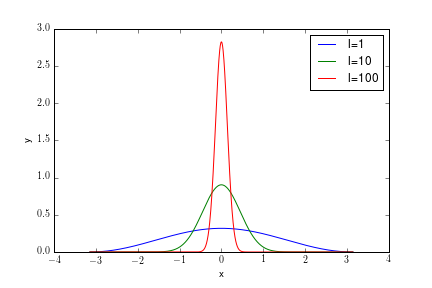
\includegraphics[width=0.40\textwidth]{figs/hk.png}}
\end{center}
\caption{\label{fig:hl} The function $h_\ell(x)$ for increasingly large values of $\ell$.}
\end{figure}

\noindent
To demonstrate the completeness of sines and cosines\footnote{This proof taken from http://web.mit.edu/jorloff/www/18.03-esg/notes/fourier-complete.pdf} we construct a peculiar but useful set of functions defined for $\ell=1,2,3,...$:
\begin{displaymath}
h_\ell(x) = c_\ell \left(\frac{1 + \cos(x)}{2}\right)^\ell
\end{displaymath}
We chose each factor $c_\ell$ such that:
\begin{displaymath}
\int_{-\pi}^{\pi} h_\ell(x) = 1
\end{displaymath}
The shape of $h_\ell$ is shown in Fig.~\ref{fig:hl}.  As $\ell$ increases, $h_\ell$ becomes more and more narrow at $x=0$, while the normalization is as in Equation~\ref{eqn:norm}.  It looks more and more like the delta function:
\begin{displaymath}
\lim_{\ell \to \infty} h_\ell(x) = \delta(x)
\end{displaymath}
It has one other important feature:  $h_\ell(x)$ is simply a sum of cosines of $nx$ with coefficients that don't depend on $x$.  To see how this can be, note that we can always turn a product of cosines into a sum via the trigonometric identity:
\begin{displaymath}
\cos \alpha \cos \beta = \frac{1}{2} \{\cos(\alpha - \beta) + \cos(\alpha + \beta)\}.
\end{displaymath}
So, for instance, we can write:
\begin{eqnarray*}
h_2(x) &=& \frac{c_2}{4} + \frac{c_2\cos(x)}{2}+\frac{c_2\cos^2(x)}{4} \\
           &=& \frac{c_2}{4} + \frac{c_2\cos(x)}{2}+\frac{c_2\cos(2x)}{8}
\end{eqnarray*}
This property implies that the function $h_\ell(x-a)$ for some constant $a$ is simply a sum of {\em both} sines and cosines of $nx$ with coefficients that don't depend on $x$, as:
\begin{displaymath}
\cos(nx-na) = \cos(nx)\cos(na) + \sin(nx)\sin(na).
\end{displaymath}

With this technology in hand we are ready to demonstrate the completeness of the sines and cosines.   
For simplicity, it suffices to consider only functions with period $L=2\pi$ (i.e. $k_n=n$).  The general case can then be inferred by transformation of coordinates.  Consider a real function $f(x)$ which is periodic for $L=2\pi$.  For now just define the function $F(x)$ to be the infinite series:
\begin{eqnarray}
F(x) \equiv a_0 + \sum_{n=1}^{\infty}  \left\{ a_n \, \cos(n x ) + b_n \, \sin(n x ) \right\}.
\end{eqnarray}
This is the compact form of the Fourier Series for this special case $L=2\pi$, so $k_n = n$.
We assume the coefficients are determined in the usual way:
\begin{eqnarray*}
a_n &=& \frac{2}{L} \int_{-\frac{L}{2}}^{\frac{L}{2}} 
f(x) \cos(n x) \, dx  \\
b_n &=& \frac{2}{L} \int_{-\frac{L}{2}}^{\frac{L}{2}} 
f(x) \sin(n x) \, dx.
\end{eqnarray*}
We need to show that $F(x) = f(x)$, or 
\begin{displaymath}
g(x) = F(x) - f(x) = 0
\end{displaymath}
The proof hinges on the fact that $F(x)$ and $f(x)$ have the same Fourier coefficients, so that:
\begin{eqnarray*}
\int_{-\pi}^{\pi} g(x) \sin(nx) dx &=& \int_{-\pi}^{\pi} F(x) \sin(nx) dx -  \int_{-\pi}^{\pi} f(x) \sin(nx) dx \\
&=& b_n - b_n \\
&=& 0 \\
\int_{-\pi}^{\pi} g(x) \cos(nx) dx &=& \int_{-\pi}^{\pi} F(x) \cos(nx) dx -  \int_{-\pi}^{\pi} f(x) \cos(nx) dx \\
&=& a_n - a_n \\
&=& 0 
\end{eqnarray*}
This shows that the integral of $g(x)$ times any sine or cosine is zero.  But our special function $h_\ell(x-a)$ function is just a sum of sines and cosines of $nx$ for any value of $a$.  This means that:
\begin{eqnarray*}
\int_{-\pi}^{\pi} h_\ell(x-a) g(x) dx &=& 0 \\
\end{eqnarray*}
If we take the limit as $\ell \to \infty$, we obtain:
\begin{eqnarray*}
\int_{-\pi}^{\pi} \delta(x-a) g(x) dx &=& 0 \\
g(a) &=& 0 \\
\end{eqnarray*}
Since this is true for any value of $a$, we have $g(x) = 0$ and so $F(x) = f(x)$.

\subsection{The orthogonality and completeness of the complex exponential function}

The first thing we need to show is that:
\begin{equation} \label{eqn:delta}
\frac{1}{2\pi} \int_{-\infty}^{\infty} \exp(ikx) \, dk = \delta(x)
\end{equation}
To see this we first calculate:
\begin{eqnarray*} \label{eqn:delta}
\frac{1}{2\pi} \int_{-a}^{a} \exp(ikx) \, dk &=& \frac{1}{2\pi} \, \frac{\exp(iax)-\exp(-iax)}{ix}\\
&=& \frac{1}{\pi} \, \frac{\sin(ax)}{x} \\
&=& \frac{a}{\pi} \, {\rm sinc}(ax)
\end{eqnarray*}
An integration shows that:
\begin{eqnarray}
\int_{-\infty}^{\infty} \frac{a}{\pi} \, {\rm sinc}(ax) \, dx = 1
\end{eqnarray}
exactly as needed for Equation~\ref{eqn:norm}.

Fig.~\ref{fig:sinc} shows that this function peaks at zero and becomes more and more narrow for progressively larger values of $a$.  Since it has the correct normalization, we conclude that:
\begin{eqnarray*}
\frac{1}{2\pi} \int_{-\infty}^{\infty} \exp(ikx) \, dk &=& \lim_{a\to\infty} \frac{1}{2\pi} \int_{-a}^{a} \exp(ikx) \, dk \\
&=& \lim_{a\to\infty} \frac{a}{\pi} \, {\rm sinc}(ax) \\ 
&=& \delta(x)
\end{eqnarray*}

\begin{figure}[thb]
\begin{center}
{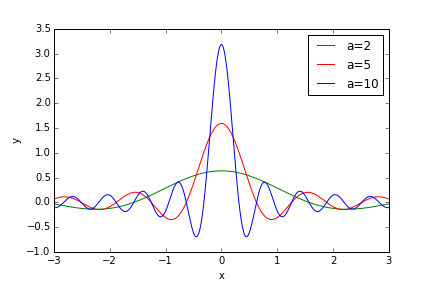
\includegraphics[width=0.40\textwidth]{figs/sinc.png}}
\end{center}
\caption{\label{fig:sinc} The function $a \, {\rm sinc}(ax)/\pi$ for progressively larger values of $a$.  As $a \to \infty$, this function approaches the delta function $\delta(x)$.}
\end{figure}

We are now fully equip to show that the complex exponential functions:
\begin{equation*}
e_k = \frac{1}{\sqrt{2\pi}} \exp(i k x)
\end{equation*}
are orthonormal.  Calculating the inner product
\begin{eqnarray*}
\braket{e_k, e_{k'}} &=& \int_{-\infty}^{\infty} \frac{1}{\sqrt{2 \pi}}  \exp(-ikx) \frac{1}{\sqrt{2 \pi}}  \exp(ik'x) \, dx \\
                               &=& \frac{1}{2 \pi} \int_{-\infty}^{\infty} \exp\{i(k'-k)x\} \, dx \\
                               &=& \delta(k-k')
\end{eqnarray*}
where we have used Equation~\ref{eqn:delta} but with the roles of $x$ and $k$ exchanged.
To prove completeness, we can now show that:
\begin{eqnarray*}
\Psi(x) &=& \int_{-\infty}^{\infty} \Psi(x') \, \delta(x-x') \, dx' \\
&=& \int_{-\infty}^{\infty} f(x') \left\{ \frac{1}{2 \pi} \int_{-\infty}^{+\infty} \exp\{ik(x-x')\} \, dk \right\} \, dx' \\
&=& \frac{1}{\sqrt{2 \pi}} \int_{-\infty}^{\infty} \left\{ \frac{1}{\sqrt{2 \pi}} \int_{-\infty}^{+\infty} f(x') \exp(-ikx') \, dx' \right\}  \exp(ikx) \, dk \\
&=& \frac{1}{\sqrt{2 \pi}} \int_{-\infty}^{\infty} \widetilde{\Psi}(k)  \exp(ikx) \, dk \\
\end{eqnarray*}
where:
\begin{eqnarray*}
\widetilde{\Psi}(k) &=& \frac{1}{\sqrt{2\pi}} \int_{-\infty}^{\infty} \Psi(x) \, \exp(-ikx) \, dx \\
\end{eqnarray*}








\end{document}



\section{Compact Form of the Fourier Series}

The Fourier Series developed above has the considerable advantage that it makes explicit the role of the sine and cosine functions as an orthonormal basis.  But it is a bit unwieldy as written.  Consider Equation~\ref{eqn:lfs} again:
\begin{eqnarray*}
f(x) = \sqrt{\frac{2}{L}} \sum_{n=0}^{\infty}  A_n \, \cos\left(\frac{2\pi n}{L} \, x \right) + \sqrt{\frac{2}{L}} \sum_{n=1}^{\infty} B_n \, \sin\left(\frac{2\pi n}{L} \, x \right) 
\end{eqnarray*}
Since $\cos(0) = 1$, the first term in the left sum is just a constant $A_0$.  It is also convenient to absorb the normalization factor $\sqrt{2/L}$ into the coefficients.  The series is therefore most often written in the much more compact form:
\begin{eqnarray}
f(x) = a_0 + \sum_{n=1}^{\infty}  \left\{ a_n \, \cos(k_n x ) + b_n \, \sin( k_n x ) \right\}\label{eqn:fs}
\end{eqnarray}
where we have introduced the wave numbers:
\begin{equation}
k_n \equiv \frac{2 \pi n}{L} \label{eqn:kn}
\end{equation}
and the new Fourier Coefficients:
\begin{eqnarray}
a_n &\equiv& \sqrt{\frac{2}{L}}  A_n = \frac{2}{L} \int_{-\frac{L}{2}}^{\frac{L}{2}} 
f(x) \cos( k_n x) \, dx \label{eqn:fca} \\
b_n &\equiv& \sqrt{\frac{2}{L}}  B_n = \frac{2}{L} \int_{-\frac{L}{2}}^{\frac{L}{2}} 
f(x) \sin( k_n x) \, dx \label{eqn:fcb}
\end{eqnarray}

\section{Fourier Series for Complex Functions}

The Fourier Series can be expressed in terms of the complex exponential by noting that:
\begin{eqnarray*}
\cos(k_n x) &=& \frac{\exp(i k_n x) + \exp(-i k_n x)}{2} \\
\sin(k_n x) &=& \frac{\exp.(i k_n x) - \exp(-i k_n x)}{2i}
\end{eqnarray*}
So that Equation~\ref{eqn:fs} can be rewritten as:
\begin{eqnarray}
f(x) &=& a_0 + \sum_{n=1}^{\infty}  \left\{ a_n \, \cos(k_n x ) + b_n \, \sin( k_n x ) \right\} \nonumber \\
&=& a_0 + \sum_{n=1}^{\infty}  \left\{ a_n \,  \frac{\exp(i k_n x) + \exp(-i k_n x)}{2} 
+ b_n \, \frac{\exp(i k_n x) - \exp(-i k_n x)}{2i} \right\} \nonumber \\
&=& a_0 + \sum_{n=1}^{\infty}  \left\{ \frac{a_n - i b_n}{2} \exp(i k_n x) + 
\frac{a_n + i b_n}{2} \exp(-i k_n x) \right\} \nonumber \\
&=& a_0 + \sum_{n=1}^{\infty}  \left\{ c_n \exp(i k_n x) + 
c_n^* \exp(-i k_n x) \right\} \label{eqn:cfsr} \label{eqn:cfsr} 
\end{eqnarray}
Where in the last step we have introduced the complex Fourier coefficient:
\begin{displaymath}
c_n \equiv \frac{a_n - i b_n}{2}.
\end{displaymath}
Note that each term of the sum in Equation~\ref{eqn:cfsr} contains two terms, with the second being the complex conjugate of the first.  Since $z+z^*$ is always a real number, the function $f(x)$ is real valued, as was our initial assumption.

If we replace our initial real function $f(x) $ with a complex valued function $\Psi(x)$ (such as a wave function in Quantum Mechanics!), the constraint that these coefficients are complex conjugates vanishes, and we can replace $c_n^*$ with new independent\footnote{If you prefer, you can construct the complex function from two real functions:  $\Psi(x) = f(x) + i g(x)$.  Either way, you have twice as many independent Fourier coefficients when the function is complex valued.} complex Fourier coefficients $d_n$.   Furthermore, the real constant $a_0$ can be replaced by a complex constant $c_0$.  
\begin{eqnarray*}
\Psi(x)  &=& c_0 + \sum_{n=1}^{\infty}  \left\{ c_n \exp(i k_n x) + 
d_n \exp(-i k_n x) \right\} \label{eqn:cfsr} \label{eqn:cfsr} 
\end{eqnarray*}
And finally, we note that we can simplify this equation even further by being quite clever, noting that 
$k_{(-n)} = -k_n$ and defining $c_{(-n)} \equiv d_n$:
\begin{eqnarray}
\Psi(x)  &=& c_0 + \sum_{n=1}^{\infty}  c_n \exp(i k_n x) + \sum_{n=1}^{\infty}  d_n \exp(-i k_n x) \nonumber \\
 &=& c_0 + \sum_{n=1}^{\infty}  c_n \exp(i k_n x) + \sum_{n=-\infty}^{-1}  c_n \exp(i k_n x) \nonumber \\
\Psi(x) &=& \sum_{n=-\infty}^{\infty} c_n \exp(i k_n x). \label{eqn:cfs}
\end{eqnarray}
Its amusing to compare the size of Equation~\ref{eqn:lfs} with Equation~\ref{eqn:cfs}, and note that the latter form is considerably more powerful.  To determine the complex Fourier coefficients we calculate:
\begin{eqnarray}
c_n &\equiv& \frac{a_n - i b_n}{2}. \nonumber \\
&=& \frac{1}{2} \left\{ 
\frac{2}{L} \int_{-\frac{L}{2}}^{\frac{L}{2}}  \Psi(x) \cos( k_n x) \, dx
-i \frac{2}{L} \int_{-\frac{L}{2}}^{\frac{L}{2}}  \Psi(x) \sin( k_n x) \, dx
\right\} \nonumber \\
&=& \frac{1}{L} \int_{-\frac{L}{2}}^{\frac{L}{2}}  \Psi(x) \left\{\cos( k_n x) - i \sin( k_n x) \right\} \, dx \nonumber \\
c_n &=& \frac{1}{L} \int_{-\frac{L}{2}}^{\frac{L}{2}}  \Psi(x) \exp(-i k_n x) \, dx \label{eqn:cfc}
\end{eqnarray}

Now look closely at Equation~\ref{eqn:cfs} and Equation~\ref{eqn:cfc} and spot the negative sign in the exponential function of the latter.  It seems something strange has happened.  Instead of the sines and cosines, we would like to think of our new orthonormal basis as the complex exponential functions 
\begin{equation}
e_n(x) \equiv \frac{1}{\sqrt{L}}\exp(i k_n x).  
\end{equation}
But to calculate the coefficient of $\exp(i k_n x)$, we integrate with respect to a {\em different} function $\exp(-i k_n x)$.  Can our vector analogy survive this?  It seems as though we are calculating the component along $\hat{x}$ by taking the dot product with $-\hat{x}$.   

It turns out that for complex valued functions, we need to modify our inner product to include complex conjugation of one of the functions:
\begin{equation}
\braket{\Psi, \phi} \equiv \int_{-\frac{L}{2}}^{\frac{L}{2}} \Psi^*(x) \phi(x) \, dx
\end{equation}
With this simple tune up, the vector analogy for complex valued functions is saved!   We still have orthonormal basis functions:
\begin{eqnarray}
\braket{e_n, e_m} &=& \frac{1}{L} \int_{-\frac{L}{2}}^{\frac{L}{2}}  \exp(-i k_n x) \exp(k_m x) \, dx \nonumber \\
&=& \delta_{nm} \label{eqn:eno}
\end{eqnarray}
(you will show this in HW Problem 2) and we still calculate the coefficient of $e_n(x)$ from the inner product:
\begin{equation}
c_n = \frac{1}{L} \braket{e_n, \Psi} = \frac{1}{L} \int_{-\frac{L}{2}}^{\frac{L}{2}}  \Psi(x) \exp(-i k_n x) \, dx
\end{equation}





\section{The Harmonic Oscillator}

\section{The Free Particle}

\section{Chapter Review}

...


\appendix



\section{The Uncertainty Principle}

Imagine that a particle is near $x=0$ with some uncertainty $\sigma_x$.  One way we might describe such a state is that the probability distribution is a Gaussian (bell-curve) distribution:
\begin{displaymath}
|\Psi(x)|^2 = N_x^2 \exp\left(-\frac{x^2}{2\sigma_x^2}\right)
\end{displaymath}
where $N_x$ is a normalization factor chosen such that 
\begin{displaymath}
\int_{-\infty}^{\infty} |\Psi(x)|^2 = 1.
\end{displaymath}
One wave function that would lead to such a probability distribution is 
\begin{displaymath}
\Psi(x) = N_x \exp\left(-\frac{x^2}{4\sigma_x^2}\right).
\end{displaymath}
Let's look at the momentum wave function for this particle:
\begin{eqnarray} 
\widetilde{\Psi}(p) &=&  \frac{1}{\sqrt{2\pi\hbar}} \int_{-\infty}^{\infty} {\Psi}(x) \exp(-ipx/\hbar) \, dx \\
&=&  \frac{N}{\sqrt{2\pi\hbar}} \int_{-\infty}^{\infty}  \exp \left(-\frac{x^2}{4\sigma_x^2} - \frac{ipx}{\hbar}\right) \, dx
\end{eqnarray}
The trick to solving this integral is called {\em completing the square}, we add and subtract the missing term needed to write this as $(x+a)^2 + b$:
\begin{eqnarray*} 
X &=&  -\frac{x^2}{4\sigma_x^2} - \frac{ipx}{\hbar} \\
&=&  -\frac{1}{4\sigma_x^2}(x^2 - 4ipx\sigma_x^2/\hbar) \\
&=&  -\frac{1}{4\sigma_x^2}(x^2 - 4ipx\sigma_x^2/\hbar  + 4i^2p^2\sigma_x^4/\hbar^2 - 4i^2p^2\sigma_x^2/\hbar^2) \\
&=&  -\frac{(x - 2 i p\sigma_x^2/\hbar)^2}{4\sigma_x^2} - p^2\sigma_x^2/\hbar^2
\end{eqnarray*}
The whole point of this is that because $x$ runs from $-\infty$ to $\infty$ we can now make a change of variables $x - 2 i p\sigma_x^2/\hbar \to x$ to clean things up dramatically:
\begin{eqnarray*} 
X &=&  -\frac{x^2}{4\sigma_x^2} - p^2\sigma_x^2/\hbar^2
\end{eqnarray*}
Our integral now becomes:
\begin{eqnarray} 
\widetilde{\Psi}(p) &=&  \frac{N}{\sqrt{2\pi\hbar}} \int_{-\infty}^{\infty}  \exp \left( -\frac{x^2}{4\sigma_x^2} - p^2\sigma_x^2/\hbar^2 \right) \, dx \nonumber \\
&=& \left\{ \frac{N}{\sqrt{2\pi\hbar}} \int_{-\infty}^{\infty}  \exp \left( -\frac{x^2}{4\sigma_x^2} \right) \right\} \exp\left( - p^2\sigma_x^2/\hbar^2 \right) \nonumber \\
&=& N_p \exp(-p^2 \sigma_x^2/\hbar^2) \label{eqn:psip}
\end{eqnarray}
Where in the last step we have noted that the term in brackets is just a constant and set $N_p=\{...\}$.

Fortunately the term in brackets ${}$ does not depend on $p$ at all... there's no need to calculate it, it will just give us a normalized momentum wave function.  We might it as well just set it to $N_p$:
Recall that we started with a wave function which had a Gaussian (bell-shaped) probability distribution with uncertainty $\sigma_x$:
\begin{displaymath}
|\Psi(x)|^2 = N_x^2 \exp\left(-\frac{x^2}{2\sigma_x^2}\right).
\end{displaymath}
We found that the momentum wave function also has a Gaussian probability distribution, if we call the uncertainty on the momentum $\sigma_p$, the probability distribution should have form the same form:
\begin{eqnarray*}
|\widetilde{\Psi}(p) |^2 &=& N_p^2 \exp\left(-\frac{p^2}{2 \sigma_p^2} \right)
\end{eqnarray*}
Comparing this to Equation~\ref{eqn:psip} we conclude:
\begin{displaymath}
\sigma_p = \frac{\hbar}{2 \sigma_x}
\end{displaymath}
or:
\begin{displaymath}
\sigma_x \sigma_p = \frac{\hbar}{2}
\end{displaymath}
Since uncertainties can always be worse than the best case, we have more generally:
\begin{displaymath}
\sigma_x \sigma_p \geq \frac{\hbar}{2}
\end{displaymath}
This is the Heisenberg uncertainty principle of quantum mechanics.  The more precisely the position is determined, the less precisely the momentum is determined, and vice versa.  It is a direct consequence of the wave like nature of matter.

This is optional reading.  A proper mathematical proof of these concepts requires about a one year course.  Fortunately, physicist are generally satisfied with informal proofs of mathematical concepts, because for us the ultimate validation is experiment!



\end{document}




